% TRR_latex_guidelines.tex V1.00, 31 August 2020

\documentclass{article}

\usepackage{arxiv}
\usepackage[numbers]{natbib}
\usepackage{moreverb,url}
\usepackage{booktabs}
\usepackage[colorlinks,bookmarksopen,bookmarksnumbered,citecolor=red,urlcolor=red]{hyperref}
\usepackage{amsmath}
\usepackage{longtable}
\usepackage{mdframed}
\usepackage{caption}
\usepackage{array}
\usepackage{todonotes}

\usepackage{rotating}

\usepackage{caption}
\captionsetup[table]{skip=10pt}

\newcommand\BibTeX{{\rmfamily B\kern-.05em \textsc{i\kern-.025em b}\kern-.08em
T\kern-.1667em\lower.7ex\hbox{E}\kern-.125emX}}

\title{Discrepancies in Closeness Centrality Formulations: Implications for reproducibility in urban network analysis.}

\author{
  %% Coauthor \\
  %% Affiliation \\
  %% Address \\
  %% \texttt{email} \\
  %% \And
  %% Coauthor \\
  %% Affiliation \\
  %% Address \\
  %% \texttt{email} \\
  %% \And
  %% Coauthor \\
  %% Affiliation \\
  %% Address \\
  %% \texttt{email} \\
}

\begin{document}
\maketitle
\todo[inline]{The authorship will be inserted after review.}
\begin{abstract}
  Street network analysis provides insights into the emergent structure of streets and the potential ramifications of spatial interventions due to associations with pedestrian movement and intensities of land uses. However, the application of street network analysis in urban planning practice presents a complex historical trajectory with nuanced distinctions in representations, methodologies, and formulations. This can lead to ambiguity in usage over time, presenting a challenge to reproducibility and the generalisation of findings.

This paper notes a divergence between commonly cited formulations for closeness centrality (\emph{Normalised Closeness}) and the form of closeness favoured by computational packages (\emph{Improved Closeness}). We hypothesise that this arises due to a widespread shift to localised forms of network analysis (based on distance thresholds), which causes \emph{Normalised Closeness} to behave counter-intuitively.  Using open datasets and an openly reproducible workflow for Madrid, Spain, we show empirically that \emph{Normalised Closeness} is weakly associated with land-use intensities and trip origin-destinations for localised network analysis, and behaves contrary to \emph{Harmonic Closeness} and \emph{Improved Closeness} which show robust associations.

We clarify the context of this methodological misunderstanding and advocate for the use of openly reproducible reference workflows and datasets to aid with reproducibility and to control for differences that might otherwise be attributable to variations in datasets, formulations, and network representations.

\end{abstract}

\noindent\textbf{Keywords:} closeness centrality; street networks; urban analytics; reproducibility; space syntax; accessibility

\section{Introduction}

Street network analysis enables the study of relationships between urban configuration and patterns of activity. Certain streets are livelier than others; land-uses cluster in particular locations; walkable configurations can become destinations in their own right \cite{Jacobs1961}. These emergent properties are difficult to anticipate for planned street networks without recourse to the incremental development typical of historical towns \cite{Alexander1967}. Network centrality measures make such properties tractable, relating the structure of street systems to characteristics such as accessibility and movement potential \cite{Hillier1984, Porta2009}. Space syntax theory, developed by Hillier and colleagues, integrated network measures with a social theory of space to analyse cities \cite{Hillier1984}, prompting wider adoption of street network analysis in urban design and planning.

Yet a documentation gap now threatens reproducibility. The closeness centrality formulas cited in published literature diverge from those implemented in widely used software packages. For global analysis on fixed graphs, this distinction may pass unnoticed. For localised analysis---where distance thresholds define varying subgraphs at each origin---the consequences are substantial. A researcher implementing the cited formula to replicate a study will obtain different results, potentially with reversed sign or negligible magnitude.

This matters because localised analysis is now standard practice. It mitigates edge effects, enables cross-city comparisons, and permits multi-scalar investigation of network properties \cite{Turner2007, van_nes_introduction_2021}. The shift from global to localised methods required adaptation of the underlying mathematics, but this transition is not well documented. Developers of packages such as \texttt{Depthmap} \cite{Hillier2012}, \texttt{Place Syntax Tool} \cite{stahle_place_2023}, and \texttt{cityseer} \cite{simons_cityseer_2023} adapted their closeness implementations accordingly, yet papers using these tools continue to cite formulations that behave differently under localised conditions.

The issue sits within a broader context of reproducibility challenges in street network analysis, including differences in network representation \cite{feng_accessibility_2022, Marshall2018}, algorithmic variations \cite{krenz_kimon_developments_2022}, and inadequate control for edge effects \cite{Gil2017}. The divergence between cited and implemented closeness formulations represents a specific, tractable instance of these challenges---one with clear mathematical explanation and practical resolution.

In this paper, we clarify the distinction between closeness formulations, explain why it matters for localised analysis, and demonstrate the behavioural differences empirically. We provide open code and data for reproducibility.

Our contribution is methodological, not substantive. We do not claim that any centrality formulation correctly captures urban accessibility, nor that correlations with land-use represent causal relationships. Rather, we demonstrate that formulations behave differently under localised analysis---a mathematical property---and use correlations with urban variables as a diagnostic tool to reveal this divergence. The theoretical argument is general; the specific correlation magnitudes serve only to show that the divergence has practical consequences.

\paragraph{What this paper adds:} We document a divergence between the closeness formulation cited in the street network analysis literature (\emph{Normalised Closeness}) and the variants implemented in computational packages (\emph{Improved Closeness}). We explain theoretically why this distinction matters for localised analysis: \emph{Closeness} exhibits sign reversal when subgraph sizes vary; \emph{Normalised Closeness} yields negligible associations; \emph{Improved} and \emph{Harmonic Closeness} scale as expected. We demonstrate these behaviours empirically and provide an openly reproducible workflow.

\paragraph{Research questions:} \textbf{RQ1:} Do different closeness formulations behave differently under localised street network analysis? \textbf{RQ2:} Are these mathematical differences empirically detectable when centrality measures are correlated with urban indicators? We hypothesise that \emph{Closeness} will exhibit sign reversal under localised analysis because it conflates subgraph size with average distance, and that \emph{Normalised Closeness} will not correct this. By contrast, \emph{Improved} and \emph{Harmonic Closeness} should scale appropriately. Section~\ref{closeness_centrality} develops this hypothesis formally; Sections~\ref{empirical-methodology}--\ref{data-analysis} demonstrate these differences empirically.

\section{Street Network Analysis}\label{network-analysis}

The intuition of networks (graphs) is that nodes (vertices) are connected by links (edges) to other nodes. For example, a social network may consist of individuals connected through relationships with one another. Network analysis can then be used to answer how connected or `relatively central' a particular person is, thus inferring their structural importance within the network. Two of the more common measures of importance are \emph{closeness centrality} \cite{Sabidussi1966}, how closely a node is located to other nodes, and \emph{betweenness centrality} \cite{Freeman1977}, how often a node provides the shortest path between other nodes. The computation of these measures involves the use of algorithms calculating \emph{shortest-paths} through the network: in the basic case, distance is topological: the number of nodes between origin and destination pairs. It is also possible to represent distance by assigning a traversal cost to the links between the nodes. For example, in street networks, these traversal costs can correspond to the lengths of streets (links) between road intersections (nodes).

To understand the contemporary context of street network analysis in practice --- and potential ramifications for closeness centrality --- it is beneficial to be aware of the literature and distinctions related to \emph{global} and \emph{localised} forms of analysis; differences in street network representation; the use of \emph{topological}, \emph{metric}, and \emph{geometric} distances as a heuristic for determining shortest paths through the network; and the impact of network topology on the robustness and comparability of results. For clarity and reproducibility, this section provides an overview of these distinctions and related background literature prior to introducing the technicalities of closeness centralities in the next section.

\subsection{Scales of Analysis}

Network centrality methods can be applied to the entirety of a network, e.g., for a given city, which is typically referred to as `global' analysis. In this case, the magnitude of the resultant network centrality is coupled to the size of the network with the implication that the larger the network, the larger the centrality values. Different boundary definitions therefore lead to fluctuating centrality values, raising some issues:
\begin{itemize}
  \item It is difficult to rigorously and consistently define boundaries from city to city. This problem is exacerbated for large urban agglomerations or when the boundaries between urban areas are not clearly delineated. One solution is to apply a technique such as network percolation \cite{Arcaute2016} to heuristically delineate boundaries;
  \item Global analysis is subject to significant ``edge-effects'', where centrality values diminish towards the edge of the network because the algorithms are constrained by the boundary. This may be manageable when using rigorous boundary definitions, but otherwise creates significant issues for comparability and generalisability \cite{Turner2007, van_nes_introduction_2021};
  \item More localised phenomena within networks cannot be directly analysed or compared because local-scale properties are masked by the global-scale characteristics of the network \cite{Porta2009, van_nes_introduction_2021}. This makes it difficult to meaningfully compare localised properties of networks between locations, particularly from the point of view of urban design and planning interventions where it is necessary to gauge local-scale impacts of design decisions.
\end{itemize}

These issues are mitigated through the use of ``localised'' network analysis which works by iteratively visiting each node using a windowing methodology to define a local catchment area for analysis \cite{Turner2007}. This intuition is conveyed in Figure~\ref{fig:moving_window}: each node is visited in turn, all other reachable nodes within a selected distance threshold are then identified and isolated from the network at large before the analysis then proceeds (using only the locally extracted sub-graph). The algorithm then steps to the next node and repeats the process until the entirety of the network has been visited.

\begin{figure}[htbp]
  \centering
  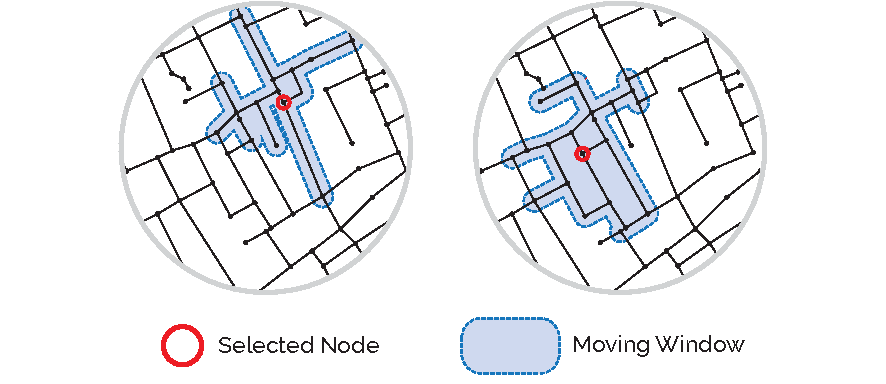
\includegraphics[width=\linewidth, keepaspectratio]{../images/moving_window.pdf}
  \caption{Moving window catchment area.}\label{fig:moving_window}
\end{figure}

Localised methods confer several advantages:
\begin{itemize}
  \item A measure computed for a given distance threshold on one network can be compared directly to the same measure and distance threshold computed for another location --- even in a different city --- because the localised boundary extents are defined in a methodologically consistent manner from location to location;
  \item Localised analysis substantially mitigates edge-effects as long as the network is adequately buffered relative to the considered distance threshold (for example, if using a 1km local catchment then a 1km buffer will eliminate edge effects);
  \item Centralities can be computed for a range of nearer or farther distance thresholds (commonly referred to as radii) to draw-out smaller or larger structures within the network. A number of different distance thresholds is ordinarily computed to understand the properties of the street network at different scales of analysis. Use of smaller distances can yield information about local-scale walkability whereas the use of larger distances can offer larger-scale insights equivalent to global methods without the aforementioned drawbacks such as edge effects.
\end{itemize}

The use of localised network analysis is therefore conventional in current practice; the remainder of this discussion and the ensuing analysis is based on the localised form of analysis. In common parlance, localised measures computed for larger radii (e.g. 10km or 20km) are sometimes sometimes termed as `global' analysis in the literature. To avoid terminological inconsistency, we refer to `localised' analysis regardless of the local distance threshold used.

\subsection{Model Representations}\label{network-representations}

The \emph{primal} representation is when intersections are represented by nodes and streets by links, thus corresponding to conceptions of streets embedded in euclidean space: intersections adopt specified coordinates connected by streets to other intersections \cite{Porta2006a}. \emph{Space Syntax}, on the other hand, emerged around the use of the \emph{dual} representation \cite{Hillier1984}. This originated with the use of \emph{axial lines} to generate a topological representation of urban space. An \emph{axial line} is an uninterrupted longest line of sight connecting convex spaces (an area where any two points can be connected by a straight line), potentially spanning multiple contiguous street segments, and distances are topological, meaning the number of steps from axial line to axial line. This is a form of \emph{dual} representation where the nodes represent street corridors and the links represent the topological steps between them. The techniques for the extrapolation of \emph{axial lines} from the street network can be complex and variable, historically leading to debates on whether it is possible to do so in an algorithmically rigorous manner \cite{Ratti2004, Turner2005a, Porta2006a}. It is important to recognise that newer and more tractable forms of dual representation have since been widely adopted by the space syntax community: \emph{fractional analysis} and the now prevalent \emph{angular segment analysis} \cite{Turner2000, Dalton2001, Turner2005a, Turner2007} forego axial lines, instead deriving the network from road centre-lines through a direct inversion of the \emph{primal} representation into its \emph{dual}, as shown in Figure~\ref{fig:primal_vs_dual}. Nodes therefore correspond to the mid-points of street segments and links typically correspond to the \emph{geometric distance} (angular change) linking them, though can also represent \emph{metric distance} (such as metres), as is typically the case for \emph{primal} representations \cite{Rosvall2005, Marshall2018, Batty2004}. Forms of distance are discussed in the following sub-section.

\begin{figure}[htbp]
  \centering
  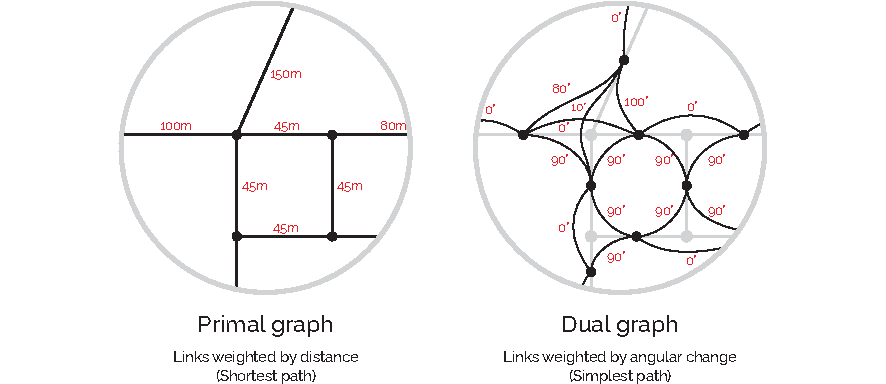
\includegraphics[width=\linewidth, keepaspectratio]{../images/primal_vs_dual.pdf}
  \caption{The \emph{primal} street network representation with \emph{metric distances} (left) and a corresponding example of a dual representation (right) with \emph{geometric distances}. Note that the dual network can be used with \emph{metric distances}.}\label{fig:primal_vs_dual}
\end{figure}

There is a large variety of potential network representations \cite{Marshall2018}, some of which can be used to analyse properties such as the connectivity of the network and its \emph{small-world} and \emph{scale-free} characteristics, emblematic of complex systems and network analysis more generally \cite{Albert2002, Porta2006a}. However, contemporary forms of street network analysis tend to adopt a pragmatic approach which leverages the widespread availability of street network datasets, typically used either directly in the \emph{primal} representation or its direct \emph{dual} inversion.

\subsection{Cost parameters}

Network links (edges) can be assigned a cost parameter to reflect distances incurred by traversing a particular link. Historically, \emph{topological distances} were used in the context of axial representations. Contemporary approaches more typically make use of \emph{metric distances} or \emph{geometric distances}. The former is ordinarily used with physical distance units such as metres whereas the latter approach is instead based on angular deviation, or in other terms the linearity of routes. Simpler routes with better lines-of-sight are therefore considered `shorter' than more convoluted routes even if the euclidean distances are greater; thus, routes requiring minimal geometric complexity are favoured to routes requiring minimal physical effort \cite{Hillier2007, Serra2019}. This tends to be the preferred distance metric in space syntax, where geometric properties of the street network are seen as important determinants in the general evolution of land-uses and the wider patterns of activities in cities \cite{Penn1998}.

The use of \emph{geometric distance} introduces an implementation nuance in that shortest-path algorithms will `bypass' sharp angular turns in cases where smaller combinations of adjacent angles can be combined instead (Figure~\ref{fig:enforced_dual}), thus making it necessary to enforce directional constraints for algorithms as they pass-through nodes during graph traversals \cite{Turner2007}. Note that unlike tailored network analysis tools such as \emph{depthmapX} \cite{turner_depthmapx_2020}, \emph{Place Syntax Tool} \cite{stahle_place_2023}, or \emph{cityseer}  \cite{simons_cityseer_2023}, generic network analysis packages typically do not take this into account and would also not necessarily return symmetrical routes if the direction of travel were reversed \cite{banino_vector-based_2018}.

\begin{figure}[htbp]
  \centering
  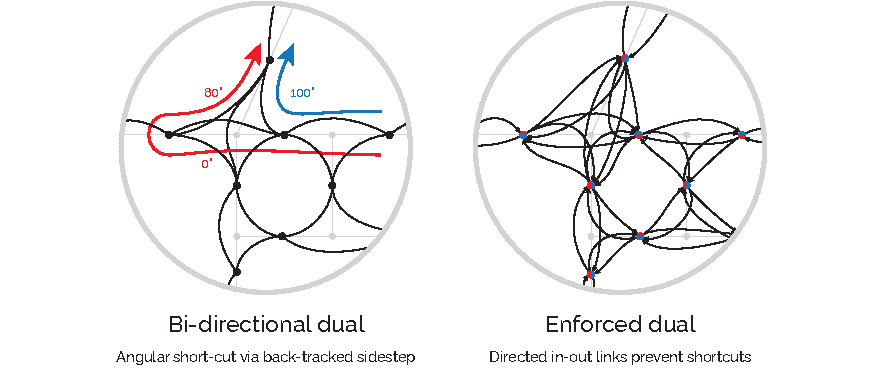
\includegraphics[width=\linewidth, keepaspectratio]{../images/enforced_dual.pdf}
  \caption{Shortest angular path side-stepping.}\label{fig:enforced_dual}
\end{figure}

\emph{Metric distance} and \emph{geometric distance} as a cost parameter are not mutually exclusive. While expressing distances differently, both are valid approaches and their interrelation is complex \cite{Barthelemy2015}. Pedestrian route choices may vary from place to place and from person to person. Shortest routes are frequently the same for either cost parameter \cite{Viana2013, Omer2018} and strong correlations are observed between them for certain distances \cite{Hillier2007, Serra2019}. Modal choice presents an additional nuance \cite{Serra2019}; research has shown strong support for \emph{geometric distances} within the context of vehicular travel, particularly at distances larger than 2000m. However, there are indications that \emph{metric distances} retain relevancy for smaller scale analysis and for non-vehicular forms of transport such as cycling \cite{Serra2019, sharmin_meta-analysis_2018}.

Note that \emph{metric distances} can be computed on the \emph{dual} and that \emph{geometric distances} can technically also be computed on the \emph{primal}, and that it is also possible to simultaneously apply multiple representations \cite{Masucci2016}.

\subsection{Distortions related to topology and geometry}

Network analysis algorithms are sensitive to the topological structure of the network, and low-quality network datasets will therefore lead to spurious results. For example, broken links will misroute shortest-path algorithms and unnecessarily complex representations of features such as intricate road intersections will introduce inflated centralities to the surrounding network.

A common problem is the conflation of the topological structure of the network with the geometrical trajectories of streets, which introduces different intensities of nodes for equivalent lengths of streets segments. For example, a straight street segment may be represented as a single link between two nodes whereas an arced street of equivalent length is often represented with additional nodes to approximate the geometric curvature of the roadway. Each additional node results in more summations when calculating centralities, consequently skewing the outcome of measures. It is therefore important to use cleaned network representations which maintain the distinction between the geometric representation of roadways and the topological structure of the network. If using more topologically complex networks from sources such as OpenStreetMap, then it is generally necessary to first clean and simplify the network. This should be done while preserving the geometry of the original street segments so that accurate distances or angular changes in direction can be measured \cite{gil_road_nodate}. In this research, these techniques are facilitated by the \texttt{cityseer-api} package \cite{simons_cityseer_2023}. There is wider interest within the network analysis community in the formalisation and standardisation of network simplification methods \cite{krenz_employing_nodate}.

Another manifestation of this phenomenon is the topological divergence between \emph{primal} and \emph{dual} representations (see Figure~\ref{fig:primal_vs_dual_structure}). Even though both derive from the same underlying structure, the outputs for the same network measures using the same cost parameters will yield different results; the \emph{dual} representation generates higher equivalent metrics due to larger quantities of nodes and links, which becomes more pronounced as the complexity of the network increases. Comparative evaluation between \emph{metric distance} measures on \emph{primal} networks and \emph{geometric distance} measures on \emph{dual} networks should be avoided because the outcomes will also reflect representational differences.

\begin{figure}[htbp]
  \centering
  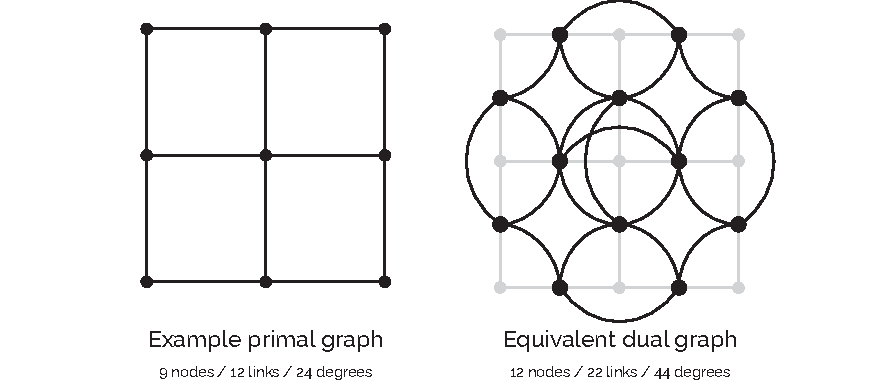
\includegraphics[width=\linewidth, keepaspectratio]{../images/primal_vs_dual_structure.pdf}
  \caption{Topological divergence of primal and dual representations.}\label{fig:primal_vs_dual_structure}
\end{figure}

\section{Closeness Centrality in Street Network Analysis}\label{closeness_centrality}

\subsection{Varying descriptions for the concept of closeness}

Application of the concept of closeness to street network analysis emerged with the development of space syntax in the late 1970s and early 1980s \cite{Hillier1984}. In this context, closeness is referred to as \emph{Integration} and implies ``to-movement'' or ``closeness'' in the general sense of the words \footnote{We here and throughout the paper refer to uncapitalised ``closeness'' in the general sense, as opposed to the capitalised form which we use to express the formal mathematical definition for \emph{Closeness}, a specific form of closeness centrality.}. In the case of the axial topological network representations used at the time, \emph{Integration} is calculated through counting the number of topological steps to surrounding nodes, taking the average, ``relativising'' the result to the size of the network, then taking the reciprocal, thereby converting the measure from farness-like to closeness-like.

After the introduction and increasing shift to angular segment analysis in the 2000s, which used street segments based on road centrelines instead of axial lines, the method for calculating \emph{Integration} was adapted to work with weighted graph edges by using summed angular deviation instead of counting topological steps. Whereas Turner at first suggested the use of \emph{Normalised Closeness} (Equation~\ref{eq:normalised_closeness}) \cite{Turner2007}, he would later suggest taking the node count divided by the average distance to the nodes \cite{turner_getting_2008}, which reflects the same intention as with the aforementioned axial integration: take \emph{Normalised Farness} (average distance), re-normalise by the number of nodes in the network, then take the reciprocal. This is reinforced in a subsequent paper \cite{Hillier2012}, where Hillier and Turner et al.\ state that the Depthmap software package calculates angular segment integration by \emph{``dividing mean angular depth by node count... and taking the reciprocal''} (where \emph{Mean Depth} refers to average distance). Closer inspection shows that this variant of closeness resembles a simplified form of the so-called \emph{Improved Closeness} (see Equations~\ref{eq:improved_closeness},~\ref{eq:used_closeness}) proposed by Wasserman and Faust \cite{Wasserman1994}, which differs from \emph{Normalised Closeness} in that it divides the node count by the \textbf{average} as opposed to \textbf{total} distance to the nodes. Notably, at least three street network analysis packages continue to use or provide this form of \emph{Improved Closeness}, including \texttt{Depthmap} \cite{Hillier2012, turner_depthmapx_2020}, the \texttt{Place Syntax Tool} \cite{stahle_place_2023}, and the \texttt{cityseer} Python package \cite{simons_cityseer_2023}.

Concurrent with the adoption of road centreline representations in the mid-2000s, and the wider interest in street network analysis more generally, researchers both within and outside of space syntax have since consistently cited \emph{Normalised Closeness} (Equation~\ref{eq:normalised_closeness}) when referring to the measure of closeness, even when these citations depend on packages such as \texttt{Depthmap} \cite{Omer2018}. Citations for non-normalised mathematical \emph{Closeness} (Equation~\ref{eq:closeness}) and even \emph{Normalised Farness} (Equation~\ref{eq:normalised_farness}) are also found. We present a selection of example references in Table~\ref{table:closeness_literature}.

\begin{table}[htbp]
  \centering

  \begin{tabular}{p{3.5cm} p{11cm}}
    \toprule
    \emph{Closeness} \& \emph{Normalised Closeness} & Representative of literature citations on street network analysis in general, which typically mention or show the formula for \emph{Normalised Closeness} \cite{crucitti_centrality_2006, Porta2009, Masucci2016, vaughan_glossary_2025, Turner2007, noauthor_segment_nodate, Porta2006} though also often discussed in the non-normalised form \cite{hutchison_network_2005, Sevtsuk2012, Cooper2015, Batty2013}. \\

    \midrule
    \emph{Improved Closeness} & Limited examples, which tend to come from technical literature or street network analysis computational packages \cite{turner_depthmapx_2020, stahle_place_2023, simons_cityseer_2023}. This form divides the node count by the \textbf{average} as opposed to \textbf{total} distance to the nodes. \\
    & \emph{``Hillier has suggested $Integ = NC / MD$ where NC is node count (i.e., the number of nodes within a network radius), and MD is mean depth of the nodes with respect to the root node.'' \cite{turner_getting_2008}} \\
    & \emph{``Angular segment analysis: The integration solution. Hillier's integration measure gives a solution that works both at low radius and radius n: $Integ = (NC * NC) / TD$'' \cite{turner_getting_2008}} (Algebraically rearranged form of $Integ = NC / MD$). \\
    & \emph{``...the current angular integration measure in Depthmap. This is found by re-dividing mean angular depth by node count... and taking the reciprocal to have high values for high integration'' \cite{Hillier2012}} \\

    \midrule
    \emph{Normalised Farness} & Limited examples, which possibly unintentionally omit mention of taking the reciprocal (which would then give \emph{Normalised Closeness}). \\
    & \emph{``Segment integration / segment angular closeness of a segment is the mean of all the angles of all the shortest paths...'' ($C_\theta$) \cite{rashid_geometry_2017, van_nes_introduction_2021}} \\
    & \emph{``Closeness...calculates the average distance from each node to all other nodes...'' \cite{Gil2017}} \\
    \bottomrule
  \end{tabular}

  \captionof{table}{Examples of different formulations attributed to the concept of closeness.}
  \label{table:closeness_literature}
\end{table}

\subsection{Research Question}

The context of our research question stems from the varying cited definitions of closeness centralities for street network analysis. At first glance, this may simply be attributable to historical evolution or different traditions of analysis; however, closer scrutiny is warranted given the divergence between cited formulations and those used by several computational packages. This has potentially significant ramifications for the comparability of findings and the reproducibility of results.

We accordingly ask whether there is a distinction in the behaviour of \emph{Improved Closeness} and \emph{Normalised Closeness} in the context of contemporary street network analysis. By ``contemporary'', we imply the use of either \emph{metric distances} (in metres) or \emph{geometric distances} (in angular deviation) on networks constructed from topologically cleaned road centreline representations, and where the measures are computed using localised methods to control for edge effects, thereby facilitating comparisons across locations and scales of analysis (see Section~\ref{network-analysis}).

We proceed with a theoretical hypothesis for why a distinction between \emph{Improved Closeness} and \emph{Normalised Closeness} is potentially meaningful for closeness centralities in street network analysis. We then conduct an empirical evaluation where we compare the behaviour of different forms of closeness centrality in the context of landuse and trip data to confirm whether the measures behave as anticipated by the hypothesis.

\subsection{Hypothesis}

As discussed in Section~\ref{network-analysis}, complications with boundary edge effects means that street network analysis has shifted to using distance localised sub-graphs for comparability across locations and scales of analysis. Turner, an early developer of road centreline street network analysis methods, expresses in a presentation given in 2008 that they (including Bill Hillier) were looking for a closeness-like formulation that is compatible with localised methods of analysis, for which a form of \emph{Improved Closeness} is proposed \cite{turner_getting_2008} (see quotations in Table~\ref{table:closeness_literature}) and subsequently adopted into \texttt{depthmap} \cite{Hillier2012}. Other than for developers of computational packages, we surmise that the distinction on workable formulations for localised closeness analysis appears not to have been broadly recognised by the wider street network analysis research community, where literature now almost universally refers to \emph{Normalised Closeness} even in the context of the predominantly used localised methods. We consequently hypothesise that \emph{Normalised Closeness} may produce counter-intuitive results for localised forms of network analysis and proceed with a theoretical description for why this may be the case.

When formally defined, the mathematical \emph{Closeness} measure
\begin{equation}\label{eq:closeness}
  Closeness_{(i)} = \frac{1}{\sum_{j\neq{i}}d_{(i,j)}}
\end{equation}
is the reciprocal of \emph{farness}
\begin{equation}\label{eq:farness}
  Farness_{(i)} = \sum_{j\neq{i}}d_{(i,j)}\, ,
\end{equation}
where \emph{Farness} is the sum of distances $d$ from node $i$ to all reachable nodes $j$ \cite{Sabidussi1966}. Mathematical \emph{Closeness} conveys how proximate node $i$ is to surrounding nodes, with the implication that high closeness centralities afford increased likelihood of access and interaction. \emph{Closeness} can be normalised by the number of nodes in the graph $N$ divided by the sum of the distances
\begin{equation}\label{eq:normalised_closeness}
  Normalised\ Closeness_{(i)} = \frac{N-1}{\sum_{j\neq{i}}d_{(i,j)}}\ ,
\end{equation}
which is the inverse of the arithmetic mean (average) of \emph{Farness}:
\begin{equation}\label{eq:normalised_farness}
  Normalised\ Farness_{(i)} = \frac{\sum_{j\neq{i}}d_{(i,j)}}{N-1}\ .
\end{equation}
When normalising, it is common to use $N-1$ to imply that the origin node $i$ is not technically counted (though this only has a notable impact on small graphs).

In the broader network analysis field, it has been shown that \emph{Harmonic Closeness} centrality \cite{Marchiori2000, Rochat2009} scales more reliably for disconnected sub-graphs, with the difference being that the division happens prior to the summation
\begin{equation}\label{eq:harmonic_closeness}
  Harmonic\ Closeness_{(i)} = \sum_{j\neq{i}}\frac{1}{d_{(i,j)}}\ .
\end{equation}

For the same reason, others have suggested \emph{Improved Closeness} centrality \cite{Wasserman1994}
\begin{equation}\label{eq:improved_closeness}
  Improved\ Closeness_{(i)} = \frac{N_{i}/{g}}{\sum_{j\neq{i}}d_{(i,j)}/{N_{i}}}\, ,
\end{equation}
which is intended for situations where a limited subset of nodes is reachable. It is defined as the ratio of the fraction of reachable nodes $N_{i}/{g}$ to the average distance to those nodes $\sum_{j\neq{i}}d_{(i,j)}/{N_{i}}$. In the context of street network analysis, the global number of nodes $g$ is ordinarily unknown; nevertheless, since this is effectively the worldwide street network and is constant for all sub-graphs, it can be proposed that the number of reachable nodes $N_{i}$ in the numerator can forego the normalisation by $g$, thus giving
\begin{equation}\label{eq:used_closeness}
  Improved\ Closeness_{(i)} = \frac{N_{i}}{\sum_{j\neq{i}}d_{(i,j)}/{N_{i}}} = \frac{N_{i}^2}{\sum_{j\neq{i}}d_{(i,j)}}\ ,
\end{equation}
which is synonymous with the formula proposed by Turner and Hillier and the variant found in several computational packages. (Note that when algebraically rearranged, the formulation can be expressed as the square of the number of reachable nodes divided by the sum of the distances to those nodes.)

The intuition of \emph{Improved Closeness} can be contrasted to \emph{Normalised Closeness} (Eq:~\ref{eq:normalised_closeness}): the number of reachable nodes is divided by the \textbf{average} distance instead of the \textbf{total} distance to the nodes. This distinction is important for localised graphs because \emph{Improved Closeness} is consequently able to scale intuitively even if the number of nodes varies: it increases either for a greater number of locally accessible nodes or if the average distance to those nodes decreases.

Figure~\ref{fig:closeness_comparisons} illustrates the implications with a simple example: Scenario B is expected to have greater closeness within an urban context than Scenario A because it is equivalently close to a greater number of nodes. Scenario C contains a more distant node and should therefore have a lower closeness centrality than Scenario B but should still be greater than A.

\begin{figure}[htbp]
  \centering
  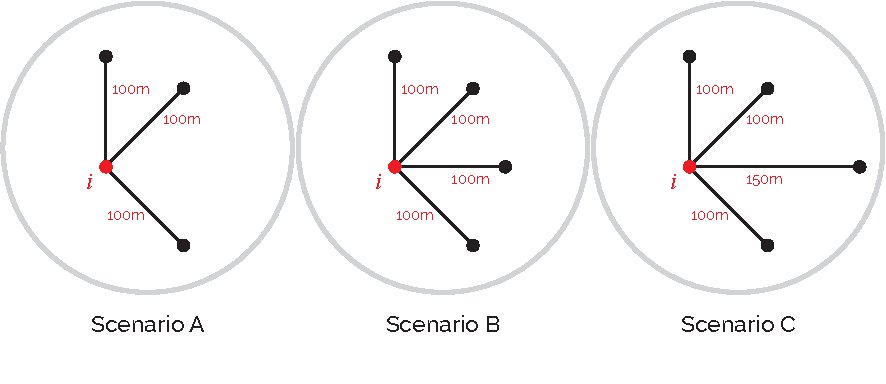
\includegraphics[width=\linewidth, keepaspectratio]{images/closeness_comparisons.pdf}
  \caption{Simple comparative localised closeness scenarios.}\label{fig:closeness_comparisons}
\end{figure}

As shown in Table~\ref{table:closeness_comparisons}, in the context of localised analysis, mathematical \emph{Closeness} behaves opposite to its intended usage because it scales differently across different quantities of nodes, decreasing from Scenario A to B and from A to C. This means that whereas mathematical \emph{Closeness} may be useful for comparing the centralities of nodes within the same graph, it behaves counter-intuitively when comparing centralities across graphs containing different numbers of nodes. \emph{Normalised Closeness} is similarly problematic for localised analysis because it now neutralises meaningful variations, such as from Scenario A to B, while also continuing to demonstrate unexpected behaviour, such as counter-intuitively decreasing from Scenario A to C. On the other hand, and as indicated in the broader network analysis literature, \emph{Harmonic Closeness} \cite{Rochat2009} and the simplified form of \emph{Improved Closeness} \cite{Wasserman1994} behave in a manner consistent with expectations across differently sized sub-graphs.

\begin{table*}[htbp]
  \centering
  \begin{tabular}{ r | r r r }
    &
    Scenario A &
    Scenario B &
    Scenario C \\
    \midrule
    \\
    $Closeness$ &
    $\frac{1}{100+100+100}=0.00\overline{3}$ &
    $\frac{1}{100+100+100+100}=0.0025$ &
    $\frac{1}{100+100+150+100}=0.00\overline{2}$ \\
    \\
    $Normalised$ &
    $\frac{3}{100+100+100}=0.01$ &
    $\frac{4}{100+100+100+100}=0.01$ &
    $\frac{4}{100+100+150+100}=0.00\overline{8}$ \\
    \\
    $Harmonic$ &
    $\frac{1}{100} + \frac{1}{100} + \frac{1}{100}=0.03$ &
    $\frac{1}{100} + \frac{1}{100} + \frac{1}{100} + \frac{1}{100}=0.04$ &
    $\frac{1}{100} + \frac{1}{100} + \frac{1}{150} + \frac{1}{100}=0.03\overline{6}$ \\
    \\
    $Improved$ &
    $\frac{3}{(100+100+100)/3}=0.03$ &
    $\frac{4}{(100+100+100+100)/4}=0.04$ &
    $\frac{4}{(100+100+150+100)/4}=0.03\overline{5}$ \\
  \end{tabular}
  \caption{Closeness comparisons.}\label{table:closeness_comparisons}
\end{table*}

Out of these, \emph{Harmonic Closeness} offers a high degree of precision because it considers the inverse of the distances independently in contrast to \emph{Improved Closeness}, which first averages the distances; yet, for the same reason, the averaging implicit with \emph{Improved Closeness} may be advantageous when working with poorer quality or unsimplified representations of street networks where individual summations may otherwise approach infinity if a network segment approaches zero length.
\section{Empirical Methodology}

We now investigate whether the empirically observed behaviour of different closeness formulations matches that anticipated from the theoretical hypothesis. Network centralities are typically associated with landuse intensities \cite{Porta2009} and travel volumes \cite{Hillier2007}; Madrid has been selected for the case study due to the availability of a high quality street network dataset accompanied by high resolution landuse premises information and an origin destination travel dataset. For full reproducibility, access to the datasets, code workflow, and related data preparation notes is provided in an open code repository.

The analysis proceeds with a range of network centralities using localised analysis from $500m$ to $10km$ so that typical behaviour can be observed at both smaller and larger scales of analysis, as is typical in the broader literature. All measures are computed on a road-centreline street network using \emph{metric} and \emph{geometric} distances applied on a dual representation of the street segments. The network is a high-quality ``cleaned'' representation, with the geometrical curvature of streets separated from the topological structure of the network.

We then provide a visual and statistical comparison on the behaviour of the aforementioned centralities:
\begin{itemize}
  \item The behaviour of the different forms is visually compared on the plotted maps;
  \item Spearman rank correlations are compared between network centralities for associations to land-use accessibility measures;
  \item Spearman rank correlations are compared between network centralities for associations to trip origin-destinations data.
\end{itemize}

The following variants of closeness are included, and are denoted as follows in the plots:
\begin{enumerate}
  \item \emph{Closeness} represents the standard non-normalised mathematical formulation of closeness centrality.
  \item \emph{Closeness $N^{1}$} indicates \emph{Normalised Closeness}, where the node count is divided by \emph{Farness}. This form is commonly cited in the street network analysis literature.
  \item \emph{Closeness $N^{1.2}$} raises the node count in the numerator to the power of 1.2. This is a form of closeness commonly used in the space syntax research community and is referred to as ``normalised" least angular integration (NAIN) \cite{Hillier2012}.
  \item \emph{Closeness $N^{2}$} squares the node count prior to the division by \emph{Farness}, and represents the version of \emph{Improved Closeness} found in computational packages. (Mathematically equivalent to dividing the node count by \emph{Normalised Farness}).
\end{enumerate}

For additional comparative context, \emph{Harmonic Closeness}, \emph{Gravity Index}, \emph{Betweenness}, and \emph{length-weighted} variants of the centralities are also computed. Where not already discussed. These are provided in the Supplementary Materials, where we also introduce continuous forms of the length-weighted measures as derived from calculus.

Accessibility \cite{Hansen1959, Handy1997, Iacono2008} to different landuses is calculated for Food \& Beverage, Retail, Services, Creative \& Entertainment, and Accommodation relative to each street segment for maximum street network distances of 100m, 200m, 500m, 1km, and 2km. A dimensionality reduction is performed on the landuse accessibility data using Principal Component Analysis (PCA), which expresses the variance contained in the datasets while removing collinearity between the variables. The centralities are then compared to stand-alone accessibilities for Food \& Beverage and Retail as well as the first principal component of the PCA, which expresses $63.6\%$ of the variance and is used as a proxy of more general landuse accessibility.

To cross-check the observations for landuse correlations, we examine whether similar patterns of observation persist when instead correlating against origin destination travel survey data. In this case, the origin-destination travel volumes for approximately 1250 travel zones for Greater Madrid is correlated to the average centrality values for all street segments falling within each zone.

The correlation plots make use of Spearman Rank $\rho$ correlation coefficients (step-wise monotonicity of the data) as opposed to Pearson's $r$ (linearity of the data) because heavily skewed datasets would otherwise require preprocessing steps (e.g.~max-log optimised boxcox transformations).

Correlations tend to be larger at greater distance thresholds because aggregation smooths  variance. This phenomenon is a characteristic of the Modifiable Areal Unit Problem \cite{Fotheringham1991} with the implication that correlations should only be directly compared between measures at the same scale of aggregation. A stronger correlation at a larger threshold is not necessarily "better" than a weaker correlation for a smaller distance, which retains a higher degree of local detail (and therefore variance).

\section{Data Sources}\label{data-methods}

Network, land use, and travel survey data are prepared for Madrid, Spain. Access to the input datasets and further detailed preparatory notes are provided in the data repository.

[The link to the data repository will be inserted after review.]

\subsection{Network Data}\hfill

The network dataset consists of an open data street network for Madrid, which is a high-quality cleaned network structure based on street centre-lines.

\textbf{Street Map of the Community of Madrid}: ``Set of roads officially approved by the municipalities of the Community of Madrid, ordered by different characteristics.''

\textbf{Source:} Madrid Open Data

\textbf{License:} \href{https://creativecommons.org/licenses/by/4.0/legalcode.es}{Creative Commons Attribution License}

\subsection{Land Use Data}\hfill

Land uses are derived from an open dataset for Madrid, consisting of 153,953 premises classed according to a schema comprising approximately 80 land use categories.

\textbf{Census of premises and their activities}: ``Microdata file of the census of premises and activities of the Madrid City Council, classified according to their type of access (street door or grouped), situation (open, closed...) and indication of the economic activity exercised and the hospitality and restaurant terraces that appear registered in said census.''

\textbf{Source:} Madrid City Council

\textbf{License:} \href{https://datos.madrid.es/portal/site/egob/menuitem.3efdb29b813ad8241e830cc2a8a409a0/?vgnextoid=108804d4aab90410VgnVCM100000171f5a0aRCRD&vgnextchannel=b4c412b9ace9f310VgnVCM100000171f5a0aRCRD&vgnextfmt=default}{License}

\subsection{Origin-Destination Travel Survey Data}\hfill

The Regional Transport Consortium of Madrid travel survey data contains approximately 200,000 origin-destination journeys encompassing approximately 1250 regions within Greater Madrid, including travel mode and travel reasons information.

\textbf{Regional Transport Consortium of Madrid Travel Survey for 2018}: Powered by CRTM

\textbf{Source:} Regional Transport Consortium of Madrid

\textbf{License:} \href{https://datos.madrid.es/egob/catalogo/aviso-legal}{License}

\section{Results}\label{data-analysis}

Following the methodology outlined in Section~\ref{empirical-methodology}, we present the results of the empirical analysis. A visual survey of the 1000m closeness centralities is plotted for \emph{metric} distance measures in Figure~\ref{fig:closeness_compare}, with \emph{geometric} distance (angular) measures shown in Figure~\ref{fig:closeness_compare_ang}. The correlation matrix for the discussed closeness centralities is shown in Figure~\ref{fig:cent_corr_matrix_close}.

\subsection{Visual Comparisons}

As illustrated in Figure~\ref{fig:closeness_compare}, \emph{Closeness} exhibits notable challenges due to its mathematical behaviour, which scales differently depending on the number of nodes under consideration. The iterative process of isolating catchments for localised calculations can therefore lead \emph{Closeness} to yield values opposite to its intended usage. \emph{Normalised Closeness} and \emph{NAIN} reduce the variance, but do not recover meaningful contrast across different street network intensities. The \emph{Improved}, \emph{Gravity}, and \emph{Harmonic} formulations behave as intended and give highly comparable results, the main differences being how these handle regions of high intensities due to differences in how nearby distances are factored into summations; see, for example, the upper right corners of the plots.

Angular variants, as illustrated in Figure~\ref{fig:closeness_compare_ang}, exhibit the same pattern for \emph{Closeness}. \emph{Normalised Closeness} and \emph{NAIN} again flatten the distribution of values, though due to the use of geometric (angular) distances, these now have a tendency to emphasise more orthogonal portions of the network with the implication that the more densely interconnected areas are less emphasised. The \emph{Improved} and \emph{Harmonic} formulations again behave as intended, once more yielding similar outputs to each other. Note that the \emph{Gravity} formulation is not applicable to geometric distances.

The above described similarities and differences between the measures are reflected in the correlation grid (Figure~\ref{fig:cent_corr_matrix_close}), where \emph{Normalised Closeness} differs markedly from the other forms and where \emph{Closeness} shows negative correlations, particularly when compared for smaller distances.

\subsection{Key Finding: Sign Reversal Across Formulations}

Before presenting detailed correlation grids, we highlight the central empirical finding. Block-bootstrap confidence intervals (accounting for spatial autocorrelation; see Section~\ref{sec:spatial_autocorr} and Table~\ref{tab:bootstrap_ci}) indicate a marked divergence in how different closeness formulations are associated with land-use intensity at localised scales:
\begin{itemize}
  \item \textbf{Closeness} is associated with a strong \emph{negative} correlation ($\rho \approx -0.70$, 95\% CI: $[-0.76, -0.64]$ at 500m), a sign reversal relative to the intended interpretation.
  \item \textbf{Normalised Closeness} ($N^1$) shows correlations near zero ($\rho \approx -0.11$, 95\% CI: $[-0.16, -0.07]$ at 500m), suggesting that simple normalisation does not address the underlying issue.
  \item \textbf{Improved Closeness} ($N^2$), \textbf{Gravity}, and \textbf{Harmonic Closeness} show consistently strong \emph{positive} correlations ($\rho \approx +0.67$, 95\% CI: $[+0.60, +0.72]$ at 500m for \emph{Improved Closeness}).
\end{itemize}
These confidence intervals account for the high spatial autocorrelation ($I \approx 0.79$--$0.84$) present in well-behaved closeness measures, which reduces the effective sample size from $N = 42{,}167$ segments to approximately 3,700 independent observations. The pattern persists across distance thresholds (500m--10km), for both metric and geometric distances, and for origin-destination trip data (Figures~\ref{fig:cent_ts_corrs},~\ref{fig:cent_ts_corrs_ang}). The following subsections present detailed correlation grids and the spatial autocorrelation analysis underpinning these estimates.

\begin{figure}[p]
  \centering
  \includegraphics[height=0.95\textheight, keepaspectratio]{plots/closeness_compare.png}
  \caption{Comparative plots of shortest metric distance closeness centralities for a 1000m catchment.}\label{fig:closeness_compare}
\end{figure}

\begin{figure}[p]
  \centering
  \includegraphics[height=0.95\textheight, keepaspectratio]{plots/closeness_compare_ang.png}
  \caption{Comparative plots of shortest geometric distance (angular) closeness centralities for a 1000m catchment. \emph{Gravity} is not applicable to geometric distances.}\label{fig:closeness_compare_ang}
\end{figure}

\begin{figure*}[htb]
  \centering
  \includegraphics[width=0.7\linewidth, keepaspectratio]{plots/cent_corr_matrix_close.pdf}
  \caption{Correlation grid of different closeness centralities.}\label{fig:cent_corr_matrix_close}
\end{figure*}

\subsection{Comparisons to Land-Use Accessibility}

Figures \ref{fig:cent_lu_corrs}, \ref{fig:cent_lu_corrs_ang}, \ref{fig:cent_lu_corrs_length_wtd}, \ref{fig:cent_lu_corrs_length_wtd_ang} represent correlation grids comparing network centralities to land-use accessibilities. Each grid can be read as follows:
\begin{itemize}
  \item The $y$ axis labels correspond to a network centrality measure.
  \item The $x$ axis labels correspond to the distance used for the localised catchment (so-called radii or moving windows) at which the network centrality measures shown on the $y$ axis have been computed, ranging from $500m$ to $10km$.
  \item The correlations shown in the individual cells correspond to the Spearman Rank correlation for a given network centrality measure ($y$ axis) at a given distance ($x$ axis) correlated to the land-use theme for a given correlation matrix (indicated in the title).
\end{itemize}

\begin{figure}[htbp]
  \centering
  \includegraphics[width=0.75\textwidth, keepaspectratio]{plots/cent_lu_corrs.pdf}
  \caption{Correlation grids comparing \emph{metric distance} network centralities to land uses.}\label{fig:cent_lu_corrs}
\end{figure}

\begin{figure}[htbp]
  \centering
  \includegraphics[width=0.75\textwidth, keepaspectratio]{plots/cent_lu_corrs_ang.pdf}
  \caption{Correlation grids comparing \emph{geometric distance} angular network centralities to land uses.}\label{fig:cent_lu_corrs_ang}
\end{figure}

\begin{figure}[htbp]
  \centering
  \includegraphics[width=0.75\textwidth, keepaspectratio]{plots/cent_lu_corrs_length_wtd.pdf}
  \caption{Correlation grids comparing length-weighted \emph{metric distance} network centralities to land uses.}\label{fig:cent_lu_corrs_length_wtd}
\end{figure}

\begin{figure}[htbp]
  \centering
  \includegraphics[width=0.75\textwidth, keepaspectratio]{plots/cent_lu_corrs_length_wtd_ang.pdf}
  \caption{Correlation grids comparing length-weighted \emph{geometric distance} angular network centralities to land uses.}\label{fig:cent_lu_corrs_length_wtd_ang}
\end{figure}

The results are broadly summarised as follows:
\begin{itemize}
  \item The density measure represents a basic count of nodes, else of street lengths for streets inside the distance thresholds for the length-weighted case. Density shows strong associations for smaller distances in spite of its simplicity, potentially indicating that for smaller catchments the overriding issue is direct access to as much of the street network as possible. The \emph{Cycles} measure, a basic count of network cycles, performs similarly.
  \item The \emph{Farness} measure is positively associated and shows stronger associations for smaller distance thresholds for reasons likely similar to density, where simple direct access to the surrounding network affords greater access to land uses. For larger distances, it lags the more complex measures because it doesn't directly consider the effective closeness of the network as the network size expands. The implication of \emph{Farness} being positively associated is that its inverse, \emph{Closeness} correlates negatively. The normalised case of either measure yields negligible associations.
  \item \emph{NAIN}, where the numerator is raised to the power of 1.2, behaves more suitably than \emph{Normalised Closeness}, though lags the \emph{Improved Closeness}, \emph{Gravity}, and \emph{Harmonic Closeness} variants which show the most consistently strong associations. The latter two appear to slightly outperform \emph{Improved Closeness}, possibly because these factor distances directly for each summation instead of first summing and then averaging the distances prior to division. However, this trend is subtle and does not likely warrant favouring one over the other.
  \item In the context of Madrid, the betweenness variants are more weakly associated to land uses than closeness-like measures. This is to be expected given Madrid's high intensities of land uses in its walkable core, which follow a fractal or `space-filling' logic utilising all available street-frontages even where not directly adjacent to the most heavily walked streets. For similar reasons, Madrid generally shows slightly weaker associations for geometric (angular) distance measures. Note that these observations may be different for other contexts (e.g. London's high streets) or for associations against pedestrian volumes as opposed to land-use intensities.
  \item The street-length weighted variants and their accompanying continuous variants exhibit similar behaviour, with generally slightly stronger associations compared to the unweighted versions.
\end{itemize}

\subsection{Comparisons to Origin-Destination Trip Data}

\begin{figure}[htbp]
  \centering
  \includegraphics[width=0.5\textwidth, keepaspectratio]{plots/cent_ts_corrs.pdf}
  \caption{Correlation grids comparing average \emph{metric distance} network centralities to trip origins and destinations for travel survey zones.}\label{fig:cent_ts_corrs}
\end{figure}

\begin{figure}[htbp]
  \centering
  \includegraphics[width=0.5\textwidth, keepaspectratio]{plots/cent_ts_corrs_ang.pdf}
  \caption{Correlation grids comparing average \emph{geometric distance} angular network centralities to trip origins and destinations for travel survey zones.}\label{fig:cent_ts_corrs_ang}
\end{figure}

Correlations of network centralities to origin-destination travel survey data, shown in Figures~\ref{fig:cent_ts_corrs} and~\ref{fig:cent_ts_corrs_ang}, largely reflect the aforementioned patterns, with \emph{Closeness} and \emph{Normalised Closeness} again showing negative or negligible associations whereas the \emph{Improved}, \emph{Gravity}, and \emph{Harmonic Closeness} versions are more strongly associated.

\subsection{Spatial Autocorrelation and Uncertainty Quantification}\label{sec:spatial_autocorr}

The spatial autocorrelation analysis (Table~\ref{tab:morans_i}) indicates a further divergence between closeness formulations. Measures that scale as anticipated --- \emph{Improved Closeness}, \emph{Gravity}, and \emph{Harmonic Closeness} --- exhibit high Moran's $I$ values ($I \approx 0.79$--$0.84$), consistent with the smooth spatial clustering typically associated with closeness centrality. Nearby street segments sharing similar network context have similarly pronounced centrality values under these formulations. In contrast, \emph{Closeness} and \emph{Normalised Closeness} exhibit lower spatial autocorrelation ($I \approx 0.18$--$0.2$ at 500m), consistent with less coherent spatial patterning.

To account for this spatial dependence when estimating uncertainty, we compute effective sample sizes and block-bootstrap confidence intervals. The effective sample size varies from approximately 3,700 for measures with high spatial coherence ($I \approx 0.84$) to 27,000 for \emph{Closeness} ($I \approx 0.21$), compared to the nominal $N = 42{,}167$ segments. The block-bootstrap procedure (Table~\ref{tab:bootstrap_ci}) uses spatially contiguous blocks to preserve autocorrelation structure, yielding conservative confidence intervals consistent with the sign-reversal pattern summarised in Section~\ref{data-analysis}: the intervals for \emph{Closeness}, \emph{Normalised Closeness}, and \emph{Improved Closeness} do not overlap, indicating that the observed divergence is statistically robust.

\subsection{Summary}

The empirical results are consistent with the theoretical hypothesis presented in Section~\ref{closeness_centrality}. \emph{Normalised Closeness}, despite being widely cited in the street network analysis literature, shows weak or negative associations with land-use accessibility and origin-destination trip volumes when computed for localised analyses. In contrast, \emph{Improved Closeness} and \emph{Harmonic Closeness} --- which scale appropriately across varying numbers of reachable nodes --- show consistently stronger associations. These findings support our contention that the divergence between cited formulations and those implemented in computational packages reflects a meaningful methodological distinction rather than notational variation.


\section{Discussion and Conclusions}\label{discussion}

The empirical results for Madrid are consistent with the theoretical hypothesis. Regarding \textbf{RQ1}, we find a meaningful distinction: mathematical \emph{Closeness} exhibits sign reversal when applied to localised analysis, correlating negatively with urban intensity where positive associations are expected. \emph{Normalised Closeness} does not correct this---it yields negligible associations. By contrast, \emph{Improved Closeness} and \emph{Harmonic Closeness} scale as expected with varying subgraph sizes. Regarding \textbf{RQ2}, these behavioural differences manifest empirically: results hold for land-use accessibility and trip counts, for length-weighted and unweighted variants, and for both metric and geometric distances.

\subsection{Who Is Affected}

Software developers have addressed this issue in practice. \texttt{DepthmapX} \cite{turner_depthmapx_2020}, \texttt{Place Syntax Tool} \cite{stahle_place_2023}, and \texttt{cityseer} \cite{simons_cityseer_2023} implement \emph{Improved Closeness} or similar variants, and some offer \emph{Harmonic Closeness} and \emph{Gravity} measures.\footnote{Some packages also provide \emph{Normalised Closeness} as an option.} Researchers using these tools obtain correct results even when citing different formulations.

The reproducibility problem affects researchers who:
\begin{itemize}
  \item Implement closeness centrality from cited formulas using generic network packages;\footnote{NetworkX provides \texttt{harmonic\_centrality} and \texttt{closeness\_centrality} with a \texttt{wf\_improved} parameter (enabled by default) implementing the Wasserman-Faust formulation, which behaves appropriately for disconnected subgraphs.}
  \item Attempt to replicate published studies without access to original code;
  \item Review or teach network centrality methods based on commonly cited formulations.
\end{itemize}

In these cases, implementing the cited \emph{Normalised Closeness} formula for localised analysis will yield different results from the original study---potentially with reversed sign or negligible magnitude.

\subsection{Implications for the Literature}

A documentation gap exists between what papers cite and what software computes. This gap likely persists because studies using appropriate software implementations produce expected results, even when citing different formulations. The mismatch becomes consequential only when attempting replication or when using generic tools.

This has implications for interpreting existing literature:
\begin{itemize}
  \item Studies using \texttt{Depthmap} or similar tools likely produced valid results regardless of cited formulations;
  \item Studies using generic network packages or custom implementations warrant scrutiny regarding which formula was actually computed;
  \item Comparative evaluations of closeness formulations should verify that implementations match cited formulas.
\end{itemize}

Earlier studies that cite \emph{Normalised Closeness} without providing open code, that select small geographic areas, or that do not buffer boundaries to control edge effects \cite{Turner2007, Porta2006} may warrant re-examination---not because their results are necessarily wrong, but because the relationship between cited methods and computed results is unclear.

\subsection{Practical Guidance}

For localised street network analysis, we recommend:
\begin{enumerate}
  \item Use closeness formulations that scale with varying subgraph sizes: \emph{Improved Closeness}, \emph{Harmonic Closeness}, or \emph{Gravity}-based measures;
  \item Document the precise formulation used, not just the generic term `closeness';
  \item Provide code or specify the software package and version to enable replication;
  \item When using generic network packages, verify that the closeness implementation is appropriate for localised analysis.
\end{enumerate}

\subsection{Limitations}

This study uses a single city (Madrid), which is appropriate because our argument is mathematical: the theoretical reasons why formulations diverge under localised analysis apply to any network where subgraph sizes vary by origin. The Madrid case demonstrates that this divergence has empirically detectable consequences. Correlation magnitudes will differ across urban contexts (e.g., cities with linear high streets, polycentric structures, or car-oriented development), but our contribution concerns the existence and direction of formulation differences, not their precise magnitude. The empirical analysis is diagnostic and cross-sectional: correlations reveal that formulations behave differently, not that any particular formulation correctly captures urban accessibility. We do not model causal relationships between centrality and land-use.

\subsection{Conclusion}

The divergence between cited closeness formulations and software implementations creates a reproducibility barrier in street network analysis. Mathematical \emph{Closeness} exhibits sign reversal under localised analysis; \emph{Normalised Closeness} yields negligible associations; \emph{Improved} and \emph{Harmonic Closeness} scale as expected under varying subgraph sizes. Researchers should use appropriate formulations for localised analysis and document computational methods precisely. We provide open code and data to support reproducibility and to serve as a reference for future methodological comparisons.


\section{Funding Statement}
\todo{Insert funding info after review.}

\section{Declaration of generative AI and AI-assisted technologies in the manuscript preparation process.}

The majority of this work was completed without the assistance of generative AI. During the final stages of preparation the authors used Claude Opus 4.5 for code, grammar, and style. After using this tool, the authors reviewed and edited the content as needed and take full responsibility for the content of the published article.

\bibliographystyle{unsrtnat}
\bibliography{references}

%% supplementary section
\clearpage  %% page break and reset figure numbering
\setcounter{figure}{0}
\makeatletter
\renewcommand{\thefigure}{S\@arabic\c@figure}
\makeatother

\section{Supplementary Materials}\label{appendix}

\subsection{Additional Centralities}\label{additional-centralities}

\subsubsection{The \emph{Gravity Index}}

The use of spatial impedance as an accessibility measure, often referred to as the \emph{Gravity Index}, shifts the emphasis to the potential flow of interactions over the street network \cite{Batty2013, Hansen1959, Rutherford1979}. Use of a spatial impedance function introduces a more configurable approach explicitly modelling spatial impedances; it reflects the potential for spatial interaction from nodes $j$ to node $i$ and --- like gravity --- how the potential for this interaction decays with distance. This typically takes the form of the negative exponential
\begin{equation}\label{eq:gravity}
  Gravity_{(i)}=\sum_{j\neq{i}}\exp(-\beta\cdot d)
\end{equation}
where the rate of decay $\beta$ (in the negative exponential) can be set to model specific trip-purposes or transportation modes to reflect people's willingness to travel a given distance $d$ to particular types of locations \cite{Sevtsuk2012, Handy1997, Iacono2008}. A variety of different impedance functions can be used, though these tend to behave similarly \cite{vale_influence_2017}.

The term \emph{Gravity Index} can be somewhat misleading: full-fledged gravity models form the basis of broader land-use and transportation modelling where the attraction of the origins and destinations are, as per gravity, taken into account. However, the \emph{Gravity Index} generally assumes equal attractions from each node to every other node and, as such, is simply a means to provide distance-weighted counts of accessible locations $j$ proximate to $i$ at the given impedance $\beta$. This approach works well for quantifying access to specific land-uses or, in the case of the street network structure, quantifying physical access from nodes $j$ to node $i$. In the context of network analysis, the strength of the decay parameter can be varied to emphasise smaller or larger structures in the network.

\begin{figure}[htp]
  \centering
  \includegraphics[width=\linewidth, keepaspectratio]{images/gravity_decay.pdf}
  \caption{Spatial impedance curves for different $\beta$ parameters. Nearer locations can be weighted more heavily than farther locations through use of the negative exponential decay function.}\label{fig:beta_decays}
\end{figure}

Gravity measures are inherently localised and do not strictly require distance cutoffs. It is nevertheless computationally advantageous to retain thresholds commensurate with distances at which the decay renders additional computation sufficiently negligible (Figure~\ref{fig:beta_decays}). For the proceeding discussion, a range of impedances is applied with the respective $\beta$ parameters anchored to distance thresholds $d_{max}$ through $\beta = 4 / d_{max}$. For example, a $100m$ distance threshold $d_{max}$ corresponds to $\beta=0.04$ and gives an average trip distance of $35m$. The distances and the corresponding impedances are selected with pedestrians in mind, where, for example, $\beta=0.005$ (800m $d_{\max}$) may represent relatively typical walking distances to bus stops \cite{Sevtsuk2016, Handy1997}. Realistically, these values vary significantly based on the purpose of the trip because pedestrians may be willing to walk much farther for purposes such as recreation and fitness than for purposes such as shopping \cite{Iacono2008}. These parameters also vary based on location: it can be argued that North American contexts are less supportive of walking \cite{Reyer2014} than European equivalents. Regardless, pedestrians tend to be unwilling to walk distances greater than a mile ($1600m$, $\beta\approx0.0025$) for non-recreational purposes and, per the exponential decay function, are more likely to walk to nearer locations than those farther away \cite{Baradaran2001, Scheurer2007, Duncan2011, Handy2001, Harris2001, Bates2007}.

\subsubsection{Betweenness centrality}

The shortest path from any node $j$ to any other node $k$ will pass through an assortment of nodes $i$, that is, unless $j$ and $k$ are directly adjacent. \emph{Betweenness}
\begin{equation}\label{eq:betweenness}
  Betweenness_{(i)} = \sum_{j\neq{i}} \sum_{k\neq{j}\neq{i}} n(j, k)\ i
\end{equation}
is the summation of shortest paths between all $(j, k)$ pairs of nodes passing through a given node $i$ \cite{Freeman1977}, and in the case of street networks conveys how likely a street is to be traversed by people travelling between other locations. Note that this measure is typically referred to as \emph{Choice} by the Space Syntax community. Localised \emph{Betweenness} only considers other $(j, k)$ node pairs within the threshold cutoff distances.

\emph{Betweenness} can be weighted by distances:
\begin{equation}\label{eq:weighted_betweenness}
  Betweenness_{(i)}=\sum_{j\neq{i}}\sum_{k\neq{j}\neq{i}} n(j, k)\ i\cdot\exp(-\beta\cdot d)\, ,
\end{equation}
in which case the negative exponential (see~\ref{eq:gravity}) can be used to reflect the notion that trips between closely located $(j, k)$ node-pairs are more likely to occur than those located farther apart, with $d$ in this case representing the corresponding trip distance for a given $(j, k)$ pair of nodes passing through node $i$.

Note that the Space Syntax methods also include the normalised least angular choice \emph{(NACH)} measure, which is described as a normalised form of \emph{Betweenness} (Choice) achieved through division by \emph{Farness} (Total Depth)
\begin{equation}\label{eq:nach}
  NACH{(i)}=\frac{\log(Betweenness + 1)}{\log(Farness + 3)}.
\end{equation} This is better described as a hybrid measure (a betweenness weighted closeness measure) rather than a normalisation, with the originators of the method stating that \emph{``it seems to combine our two measures -- depth and choice, to and through-movement" \cite{Hillier2012}}. The measure is ordinarily shown with the addition of constants in both the numerator and denominator to guard against situations such as taking the $log$ of a number less than 1.

\subsubsection{Length-weighting}
Topological distortions due to varying intensities of nodes can exaggerate the outcome of centrality measures. It is therefore common to see the nodes weighted by factors such as street lengths \cite{Turner2005a, Turner2007} or the number of adjacent buildings \cite{Sevtsuk2012}. The implication is that greater exposure to street lengths offers a greater potential for interaction, with the contribution of unusually high concentrations of nodes tempered by correspondingly shorter street segments and vice-versa. In practical terms, assuming the use of the dual representation, the length of the primal street segment is assigned to the dual node, with the nodes weighted accordingly during the calculation of the centrality measure. For example, in the case of \emph{Harmonic Closeness} the $1$ in the numerator is replaced by the length of the segment $l$:
\begin{equation}\label{eq:harmonic_length_weighted}
  HC_{(i)} = \sum_{j\neq{i}}\frac{l}{d_{(i,j)}}\, .
\end{equation}

An alternative is to use the integral of \emph{Harmonic Closeness}. The integral for $f(x)=1/d$ takes the form
\begin{equation}
  \int_{a}^{b}\ f(x)\ dx = \ln(b) - \ln(a)
\end{equation}
and can be applied to sum the `area under the (spatial impedance) curve' for the respective lower and upper segment bounds $a$ and $b$ for all reachable segments $S$:
\begin{equation}\label{eq:harmonic_integral}
  HC_{(i)} = \sum_{(a, b)}^{S} \int_{a}^{b}\ f(x)\ dx = \sum_{(a, b)}^{S}\ \ln(b) - \ln(a)\, .
\end{equation}
This allows spatial impedances to increase continuously. For example, the contribution of a 10m street segment adjacent to the origin is now found as $\ln(10) = 2.303$ and a segment from $10m$ to $20m$ distant is found as $\ln(20) - \ln(10) = 0.693$. As shown in Figure~\ref{fig:closeness_comparisons_length_weighted} and Table~\ref{table:closeness_comparisons_length_weighted}, the continuous form remains consistent regardless of how many times street lengths are split at intervening nodes.

\begin{figure}[htp]
  \centering
  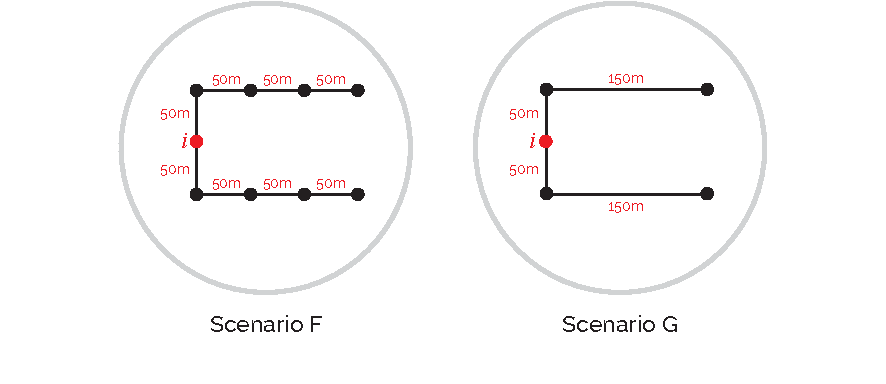
\includegraphics[width=\linewidth, keepaspectratio]{images/closeness_comparisons_length_weighted.pdf}
  \caption{Length weighted closeness formulations comparing for varied node intensities.}\label{fig:closeness_comparisons_length_weighted}
\end{figure}

\begin{table*}[htp]
  \centering
  \begin{tabular}{ r | r r }
    &
    $length\ wt.\ HC_{(i)} = \sum_{j\neq{i}}\frac{l}{d_{(i,j)}}$ &
    $Harmonic\ C_{(i)} (0, x) = \int_{0}^{x} \ln(x)\ dx$ \\
    \midrule
    \\
    Scenario F &
    $(\frac{50}{50} + \frac{50}{100} + \frac{50}{150} + \frac{25}{200})*2 = 3.92$ &
    $(simplified)\ \ln(200) * 2 = 10.60$ \\
    \\
    Scenario G &
    $(\frac{100}{50} + \frac{75}{200})*2 = 4.75$ &
    $(simplified)\  \ln(200) * 2 = 10.60$ \\
  \end{tabular}
  \caption{Length weighted closeness formulations comparing street-length weighted \emph{Harmonic Closeness} and a continuous form of \emph{Harmonic Closeness}. Continuous forms remain consistent regardless of the number of subdivisions.}\label{table:closeness_comparisons_length_weighted}
\end{table*}

Note that the continuous form of \emph{Harmonic Closeness} suggested per Equation~\ref{eq:harmonic_integral} cannot be used with \emph{geometric distance} (angular) impedances, which do not increase continuously.

As with closeness centrality, it may be preferable to use the gravity index in a continuous form. In this case, gravity is computed as the area under the curve for all reachable segments $S$ for the respective lower and upper segment bounds $a$ and $b$ at the specified impedance $\beta$:
\begin{equation}\label{eq:gravity_continuous}
  G_{(i)} = \sum_{(a, b)}^{S} \int_{a}^{b}\ f(x)\ dx = \sum_{(a, b)}^{S}\ \frac{\exp(-\beta\cdot b) -\exp(-\beta\cdot a)}{-\beta}.
\end{equation}
\subsection{Additional Figures and Tables}\label{additional-figures}

\begin{figure*}[htb]
  \centering
  \includegraphics[width=\linewidth, keepaspectratio]{plots/pca_corr_matrix.pdf}
  \caption{PCA loadings matrix.}\label{fig:pca_loadings}
\end{figure*}

\subsubsection{Descriptive Statistics Tables}

\textit{Note on closeness centrality values:} The closeness centrality measures exhibit small absolute values because they are computed as the inverse of \emph{Farness} or \emph{Normalised Farness} where the number of reachable nodes is divided by the total cumulative distance (in meters). For example, with a 500m catchment containing 100 nodes and 28,000 meters of cumulative farness, \emph{Closeness} gives $1 / 28,000 = 0.000036$ and \emph{Normalised Closeness} $100 / 28,000 = 0.00357$. These small values are mathematically correct and do not affect statistical analyses because Spearman rank correlations are based on rank order.

\begin{table}[htb]
  \centering
  \small
  \caption{Descriptive statistics for land use variables.}\label{tab:desc_landuse}
  \begin{tabular}{lrlllllll}
\toprule
 & N & Mean & Median & Q1 & Q3 & IQR & Min & Max \\
\midrule
pca\_1 & 42167 & -6.89e-04 & -0.439 & -3.177 & 2.809 & 5.986 & -5.900 & 10.000 \\
food\_bev\_200 & 42167 & 0.925 & 0.265 & 0.00e+00 & 1.134 & 1.134 & 0.00e+00 & 21 \\
retail\_200 & 42167 & 1.997 & 0.461 & 0.00e+00 & 2.328 & 2.328 & 0.00e+00 & 88 \\
\bottomrule
\end{tabular}

\end{table}

\begin{table}[htb]
  \centering
  \small
  \caption{Descriptive statistics for centrality measures.}\label{tab:desc_centrality}
  \begin{tabular}{lrlllllll}
\toprule
 & N & Mean & Median & Q1 & Q3 & IQR & Min & Max \\
\midrule
density\_500 & 42167 & 100 & 86 & 49 & 144 & 95 & 0.00e+00 & 367 \\
density\_1000 & 42167 & 352 & 330 & 192 & 496 & 304 & 0.00e+00 & 1092 \\
density\_2000 & 42167 & 1242 & 1199 & 796 & 1771 & 975 & 0.00e+00 & 2614 \\
density\_5000 & 42167 & 7078 & 7161 & 4790 & 9549 & 4759 & 0.00e+00 & 13191 \\
density\_10000 & 42167 & 25667 & 26803 & 21574 & 30862 & 9288 & 0.00e+00 & 36199 \\
far\_500 & 42167 & 32418 & 28121 & 15814 & 47338 & 31523 & 0.00e+00 & 122029 \\
far\_1000 & 42167 & 227738 & 216367 & 123304 & 316214 & 192910 & 0.00e+00 & 721591 \\
far\_2000 & 42167 & 1603791 & 1554475 & 978723 & 2329708 & 1350985 & 0.00e+00 & 3296895 \\
far\_5000 & 42167 & 23277712 & 23682352 & 15904454 & 30917964 & 15013510 & 0.00e+00 & 44062764 \\
far\_10000 & 42167 & 165974864 & 174153936 & 144394816 & 194249440 & 49854624 & 0.00e+00 & 223477152 \\
far\_norm\_500 & 41537 & 326 & 328 & 310 & 344 & 34 & 79 & 500 \\
far\_norm\_1000 & 42008 & 647 & 652 & 613 & 684 & 72 & 223 & 1000 \\
far\_norm\_2000 & 42147 & 1289 & 1296 & 1213 & 1378 & 165 & 532 & 1987 \\
far\_norm\_5000 & 42163 & 3295 & 3283 & 3168 & 3421 & 253 & 1422 & 4627 \\
far\_norm\_10000 & 42163 & 6552 & 6510 & 6204 & 6817 & 614 & 5290 & 9101 \\
closeness\_500 & 41537 & 8.05e-05 & 3.49e-05 & 2.10e-05 & 6.12e-05 & 4.02e-05 & 8.19e-06 & 6.97e-03 \\
closeness\_1000 & 42167 & 1.40e-05 & 4.59e-06 & 3.14e-06 & 8.01e-06 & 4.86e-06 & 0.00e+00 & 2.67e-03 \\
closeness\_2000 & 42147 & 1.95e-06 & 6.43e-07 & 4.29e-07 & 1.02e-06 & 5.92e-07 & 3.03e-07 & 5.77e-04 \\
closeness\_5000 & 42163 & 9.91e-08 & 4.22e-08 & 3.23e-08 & 6.29e-08 & 3.05e-08 & 2.27e-08 & 1.05e-04 \\
closeness\_10000 & 42163 & 7.50e-09 & 5.74e-09 & 5.15e-09 & 6.92e-09 & 1.78e-09 & 4.47e-09 & 1.60e-06 \\
close\_N1\_500 & 41537 & 3.10e-03 & 3.05e-03 & 2.91e-03 & 3.23e-03 & 3.17e-04 & 2.00e-03 & 1.27e-02 \\
close\_N1\_1000 & 42167 & 1.56e-03 & 1.53e-03 & 1.46e-03 & 1.63e-03 & 1.71e-04 & 0.00e+00 & 4.49e-03 \\
close\_N1\_2000 & 42147 & 7.85e-04 & 7.72e-04 & 7.26e-04 & 8.25e-04 & 9.90e-05 & 5.03e-04 & 1.88e-03 \\
close\_N1\_5000 & 42163 & 3.06e-04 & 3.05e-04 & 2.92e-04 & 3.16e-04 & 2.34e-05 & 2.16e-04 & 7.03e-04 \\
close\_N1\_10000 & 42163 & 1.53e-04 & 1.54e-04 & 1.47e-04 & 1.61e-04 & 1.45e-05 & 1.10e-04 & 1.89e-04 \\
close\_N1.2\_500 & 41537 & 7.48e-03 & 7.59e-03 & 6.72e-03 & 8.41e-03 & 1.69e-03 & 2.00e-03 & 1.46e-02 \\
close\_N1.2\_1000 & 42167 & 4.85e-03 & 4.92e-03 & 4.38e-03 & 5.47e-03 & 1.09e-03 & 0.00e+00 & 1.01e-02 \\
close\_N1.2\_2000 & 42147 & 3.16e-03 & 3.21e-03 & 2.90e-03 & 3.52e-03 & 6.23e-04 & 5.03e-04 & 4.98e-03 \\
close\_N1.2\_5000 & 42163 & 1.76e-03 & 1.81e-03 & 1.65e-03 & 1.94e-03 & 2.91e-04 & 3.05e-04 & 2.15e-03 \\
close\_N1.2\_10000 & 42163 & 1.16e-03 & 1.18e-03 & 1.09e-03 & 1.27e-03 & 1.80e-04 & 3.14e-04 & 1.37e-03 \\
close\_N2\_500 & 41537 & 0.312 & 0.272 & 0.158 & 0.447 & 0.289 & 2.00e-03 & 1.172 \\
close\_N2\_1000 & 42167 & 0.549 & 0.509 & 0.298 & 0.777 & 0.479 & 0.00e+00 & 1.728 \\
close\_N2\_2000 & 42147 & 0.969 & 0.946 & 0.609 & 1.336 & 0.726 & 5.03e-04 & 2.264 \\
close\_N2\_5000 & 42163 & 2.159 & 2.180 & 1.451 & 2.964 & 1.513 & 9.25e-04 & 3.954 \\
close\_N2\_10000 & 42163 & 3.982 & 4.137 & 3.208 & 4.905 & 1.697 & 1.47e-02 & 6.007 \\
harmonic\_500 & 42167 & 0.407 & 0.354 & 0.201 & 0.583 & 0.382 & 0.00e+00 & 1.721 \\
harmonic\_1000 & 42167 & 0.747 & 0.685 & 0.408 & 1.059 & 0.651 & 0.00e+00 & 2.532 \\
harmonic\_2000 & 42167 & 1.343 & 1.315 & 0.834 & 1.838 & 1.004 & 0.00e+00 & 3.564 \\
harmonic\_5000 & 42167 & 3.011 & 3.025 & 2.071 & 4.110 & 2.038 & 0.00e+00 & 6.155 \\
harmonic\_10000 & 42167 & 5.524 & 5.730 & 4.291 & 6.952 & 2.661 & 0.00e+00 & 9.433 \\
gravity\_500 & 42167 & 12 & 10 & 5.901 & 17 & 11 & 0.00e+00 & 47 \\
gravity\_1000 & 42167 & 44 & 40 & 23 & 63 & 40 & 0.00e+00 & 154 \\
gravity\_2000 & 42167 & 157 & 152 & 93 & 216 & 124 & 0.00e+00 & 436 \\
gravity\_5000 & 42167 & 856 & 840 & 569 & 1189 & 621 & 0.00e+00 & 1688 \\
gravity\_10000 & 42167 & 3169 & 3252 & 2312 & 4135 & 1823 & 0.00e+00 & 5272 \\
\bottomrule
\end{tabular}

\end{table}

\begin{table}[htb]
  \centering
  \small
  \caption{Descriptive statistics for length-weighted centrality measures.}\label{tab:desc_centrality_lw}
  \begin{tabular}{lrlllllll}
\toprule
 & N & Mean & Median & Q1 & Q3 & IQR & Min & Max \\
\midrule
lw\_density\_500 & 42167 & 7348 & 7184 & 4856 & 9915 & 5059 & 0.00e+00 & 18311 \\
lw\_density\_1000 & 42167 & 28119 & 28248 & 19274 & 36788 & 17514 & 0.00e+00 & 64442 \\
lw\_density\_2000 & 42167 & 108908 & 108452 & 79721 & 146356 & 66635 & 0.00e+00 & 195076 \\
lw\_density\_5000 & 42167 & 690422 & 713402 & 531238 & 875962 & 344724 & 0.00e+00 & 1141834 \\
lw\_density\_10000 & 42167 & 2659032 & 2759148 & 2332424 & 3079680 & 747256 & 0.00e+00 & 3581994 \\
lw\_far\_500 & 42167 & 2446879 & 2390021 & 1592962 & 3301552 & 1708590 & 0.00e+00 & 6266275 \\
lw\_far\_1000 & 42167 & 18561794 & 18738480 & 12520390 & 24216358 & 11695968 & 0.00e+00 & 43358996 \\
lw\_far\_2000 & 42167 & 144247104 & 144698080 & 104013600 & 193948736 & 89935136 & 0.00e+00 & 257134432 \\
lw\_far\_5000 & 42167 & 2311166464 & 2394943744 & 1786027776 & 2902958592 & 1116930816 & 0.00e+00 & 3842761216 \\
lw\_far\_10000 & 42167 & 17492131840 & 18184536064 & 15647161344 & 19928051712 & 4280890368 & 0.00e+00 & 22876850176 \\
lw\_far\_norm\_500 & 41537 & 334 & 334 & 321 & 346 & 24 & 79 & 500 \\
lw\_far\_norm\_1000 & 42008 & 661 & 662 & 635 & 685 & 49 & 345 & 1000 \\
lw\_far\_norm\_2000 & 42147 & 1322 & 1324 & 1274 & 1375 & 101 & 764 & 1987 \\
lw\_far\_norm\_5000 & 42163 & 3356 & 3342 & 3277 & 3434 & 157 & 2420 & 4625 \\
lw\_far\_norm\_10000 & 42163 & 6626 & 6579 & 6392 & 6821 & 430 & 6154 & 8590 \\
lw\_closeness\_500 & 41537 & 6.98e-07 & 4.14e-07 & 3.01e-07 & 6.13e-07 & 3.11e-07 & 1.60e-07 & 4.33e-04 \\
lw\_closeness\_1000 & 42008 & 9.47e-08 & 5.32e-08 & 4.12e-08 & 7.94e-08 & 3.81e-08 & 2.31e-08 & 1.99e-04 \\
lw\_closeness\_2000 & 42147 & 1.06e-08 & 6.91e-09 & 5.16e-09 & 9.61e-09 & 4.45e-09 & 3.89e-09 & 1.42e-05 \\
lw\_closeness\_5000 & 42163 & 5.55e-10 & 4.18e-10 & 3.44e-10 & 5.60e-10 & 2.15e-10 & 2.60e-10 & 7.09e-08 \\
lw\_closeness\_10000 & 42163 & 6.26e-11 & 5.50e-11 & 5.02e-11 & 6.39e-11 & 1.37e-11 & 4.37e-11 & 2.27e-09 \\
lw\_close\_N1\_500 & 41537 & 3.01e-03 & 3.00e-03 & 2.89e-03 & 3.11e-03 & 2.19e-04 & 2.00e-03 & 1.27e-02 \\
lw\_close\_N1\_1000 & 42008 & 1.52e-03 & 1.51e-03 & 1.46e-03 & 1.57e-03 & 1.13e-04 & 1.00e-03 & 2.90e-03 \\
lw\_close\_N1\_2000 & 42147 & 7.60e-04 & 7.55e-04 & 7.27e-04 & 7.85e-04 & 5.79e-05 & 5.03e-04 & 1.31e-03 \\
lw\_close\_N1\_5000 & 42163 & 2.99e-04 & 2.99e-04 & 2.91e-04 & 3.05e-04 & 1.40e-05 & 2.16e-04 & 4.13e-04 \\
lw\_close\_N1\_10000 & 42163 & 1.51e-04 & 1.52e-04 & 1.47e-04 & 1.56e-04 & 9.85e-06 & 1.16e-04 & 1.62e-04 \\
lw\_close\_N1.2\_500 & 41537 & 1.75e-02 & 1.79e-02 & 1.65e-02 & 1.91e-02 & 2.65e-03 & 2.99e-03 & 3.71e-02 \\
lw\_close\_N1.2\_1000 & 42008 & 1.16e-02 & 1.18e-02 & 1.09e-02 & 1.26e-02 & 1.70e-03 & 1.41e-03 & 1.67e-02 \\
lw\_close\_N1.2\_2000 & 42147 & 7.59e-03 & 7.74e-03 & 7.16e-03 & 8.19e-03 & 1.03e-03 & 1.03e-03 & 9.17e-03 \\
lw\_close\_N1.2\_5000 & 42163 & 4.34e-03 & 4.43e-03 & 4.14e-03 & 4.69e-03 & 5.49e-04 & 1.24e-03 & 4.97e-03 \\
lw\_close\_N1.2\_10000 & 42163 & 2.90e-03 & 2.94e-03 & 2.78e-03 & 3.10e-03 & 3.13e-04 & 1.14e-03 & 3.28e-03 \\
lw\_close\_N2\_500 & 41537 & 22 & 22 & 15 & 30 & 15 & 1.47e-02 & 55 \\
lw\_close\_N2\_1000 & 42008 & 43 & 43 & 29 & 56 & 27 & 5.19e-03 & 96 \\
lw\_close\_N2\_2000 & 42147 & 83 & 83 & 60 & 109 & 49 & 1.78e-02 & 155 \\
lw\_close\_N2\_5000 & 42163 & 207 & 212 & 157 & 265 & 108 & 1.360 & 340 \\
lw\_close\_N2\_10000 & 42163 & 405 & 420 & 346 & 479 & 133 & 7.206 & 569 \\
lw\_harmonic\_500 & 42167 & 28 & 27 & 18 & 38 & 19 & 0.00e+00 & 74 \\
lw\_harmonic\_1000 & 42167 & 56 & 55 & 38 & 73 & 35 & 0.00e+00 & 132 \\
lw\_harmonic\_2000 & 42167 & 109 & 111 & 80 & 142 & 62 & 0.00e+00 & 219 \\
lw\_harmonic\_5000 & 42167 & 275 & 278 & 211 & 355 & 144 & 0.00e+00 & 463 \\
lw\_harmonic\_10000 & 42167 & 540 & 557 & 453 & 647 & 194 & 0.00e+00 & 799 \\
lw\_gravity\_500 & 42167 & 818 & 803 & 532 & 1112 & 580 & 0.00e+00 & 2166 \\
lw\_gravity\_1000 & 42167 & 3273 & 3231 & 2231 & 4358 & 2127 & 0.00e+00 & 7872 \\
lw\_gravity\_2000 & 42167 & 12701 & 12858 & 9125 & 16376 & 7251 & 0.00e+00 & 26269 \\
lw\_gravity\_5000 & 42167 & 77914 & 78117 & 59244 & 102658 & 43414 & 0.00e+00 & 131299 \\
lw\_gravity\_10000 & 42167 & 309890 & 319353 & 251567 & 383456 & 131889 & 0.00e+00 & 465867 \\
\bottomrule
\end{tabular}

\end{table}

\begin{table}[htb]
  \centering
  \small
  \caption{Descriptive statistics for angular centrality measures.}\label{tab:desc_centrality_ang}
  \begin{tabular}{lrlllllll}
\toprule
 & N & Mean & Median & Q1 & Q3 & IQR & Min & Max \\
\midrule
far\_500\_ang & 42167 & 260 & 209 & 112 & 375 & 263 & 0.00e+00 & 1592 \\
far\_1000\_ang & 42167 & 1300 & 1144 & 627 & 1836 & 1208 & 0.00e+00 & 7665 \\
far\_2000\_ang & 42167 & 6462 & 6209 & 3887 & 8985 & 5098 & 0.00e+00 & 27812 \\
far\_5000\_ang & 42167 & 51751 & 53623 & 30026 & 70395 & 40369 & 0.00e+00 & 165195 \\
far\_10000\_ang & 42167 & 355383 & 372069 & 282992 & 429857 & 146865 & 0.00e+00 & 802588 \\
far\_norm\_500\_ang & 41537 & 3.054 & 2.935 & 2.393 & 3.584 & 1.192 & 9.03e-03 & 12 \\
far\_norm\_1000\_ang & 42008 & 4.665 & 4.555 & 3.794 & 5.393 & 1.600 & 5.06e-02 & 14 \\
far\_norm\_2000\_ang & 42147 & 7.248 & 7.069 & 6.121 & 8.148 & 2.027 & 0.384 & 21 \\
far\_norm\_5000\_ang & 42163 & 12 & 12 & 11 & 14 & 2.625 & 2.412 & 37 \\
far\_norm\_10000\_ang & 42163 & 19 & 19 & 17 & 21 & 3.574 & 9.871 & 48 \\
closeness\_500\_ang & 41537 & 3.18e-02 & 4.71e-03 & 2.64e-03 & 8.64e-03 & 6.00e-03 & 6.28e-04 & 111 \\
closeness\_1000\_ang & 42167 & 4.85e-03 & 8.67e-04 & 5.41e-04 & 1.58e-03 & 1.04e-03 & 0.00e+00 & 20 \\
closeness\_2000\_ang & 42147 & 7.18e-04 & 1.61e-04 & 1.11e-04 & 2.57e-04 & 1.46e-04 & 3.60e-05 & 2.603 \\
closeness\_5000\_ang & 42163 & 4.67e-05 & 1.86e-05 & 1.42e-05 & 3.33e-05 & 1.91e-05 & 6.05e-06 & 8.80e-02 \\
closeness\_10000\_ang & 42163 & 3.64e-06 & 2.69e-06 & 2.33e-06 & 3.53e-06 & 1.21e-06 & 1.25e-06 & 5.11e-04 \\
close\_N1\_500\_ang & 41537 & 0.385 & 0.341 & 0.279 & 0.418 & 0.139 & 8.33e-02 & 111 \\
close\_N1\_1000\_ang & 42167 & 0.235 & 0.219 & 0.185 & 0.263 & 7.84e-02 & 0.00e+00 & 20 \\
close\_N1\_2000\_ang & 42147 & 0.147 & 0.141 & 0.123 & 0.163 & 4.06e-02 & 4.86e-02 & 2.603 \\
close\_N1\_5000\_ang & 42163 & 8.36e-02 & 8.29e-02 & 7.40e-02 & 9.19e-02 & 1.79e-02 & 2.67e-02 & 0.415 \\
close\_N1\_10000\_ang & 42163 & 5.33e-02 & 5.28e-02 & 4.81e-02 & 5.80e-02 & 9.97e-03 & 2.06e-02 & 0.101 \\
close\_N1.2\_500\_ang & 41537 & 0.851 & 0.817 & 0.654 & 0.986 & 0.332 & 0.147 & 111 \\
close\_N1.2\_1000\_ang & 42167 & 0.677 & 0.670 & 0.548 & 0.794 & 0.245 & 0.00e+00 & 20 \\
close\_N1.2\_2000\_ang & 42147 & 0.545 & 0.545 & 0.458 & 0.629 & 0.171 & 8.87e-02 & 2.603 \\
close\_N1.2\_5000\_ang & 42163 & 0.433 & 0.436 & 0.371 & 0.497 & 0.126 & 9.17e-02 & 0.789 \\
close\_N1.2\_10000\_ang & 42163 & 0.379 & 0.380 & 0.338 & 0.424 & 8.69e-02 & 8.04e-02 & 0.665 \\
close\_N2\_500\_ang & 41537 & 28 & 26 & 14 & 40 & 25 & 0.212 & 111 \\
close\_N2\_1000\_ang & 42167 & 60 & 57 & 32 & 83 & 51 & 0.00e+00 & 231 \\
close\_N2\_2000\_ang & 42147 & 127 & 116 & 72 & 177 & 105 & 9.12e-02 & 378 \\
close\_N2\_5000\_ang & 42163 & 358 & 343 & 187 & 510 & 322 & 0.382 & 933 \\
close\_N2\_10000\_ang & 42163 & 1024 & 1023 & 775 & 1317 & 542 & 3.257 & 2332 \\
harmonic\_500\_ang & 42167 & 24 & 22 & 12 & 33 & 21 & 0.00e+00 & 90 \\
harmonic\_1000\_ang & 42167 & 56 & 53 & 31 & 78 & 47 & 0.00e+00 & 208 \\
harmonic\_2000\_ang & 42167 & 128 & 120 & 75 & 177 & 102 & 0.00e+00 & 369 \\
harmonic\_5000\_ang & 42167 & 380 & 366 & 211 & 533 & 322 & 0.00e+00 & 951 \\
harmonic\_10000\_ang & 42167 & 1122 & 1123 & 835 & 1434 & 598 & 0.00e+00 & 2542 \\
\bottomrule
\end{tabular}

\end{table}

\begin{table}[htb]
  \centering
  \small
  \caption{Descriptive statistics for length-weighted angular centrality measures.}\label{tab:desc_centrality_lw_ang}
  \begin{tabular}{lrlllllll}
\toprule
 & N & Mean & Median & Q1 & Q3 & IQR & Min & Max \\
\midrule
lw\_far\_500\_ang & 42167 & 18826 & 17213 & 10848 & 25695 & 14847 & 0.00e+00 & 84449 \\
lw\_far\_1000\_ang & 42167 & 101824 & 97161 & 63036 & 136294 & 73258 & 0.00e+00 & 470177 \\
lw\_far\_2000\_ang & 42167 & 555098 & 555054 & 384851 & 733383 & 348533 & 0.00e+00 & 1902248 \\
lw\_far\_5000\_ang & 42167 & 4896063 & 5050740 & 3259989 & 6327224 & 3067235 & 0.00e+00 & 14512521 \\
lw\_far\_10000\_ang & 42167 & 35232836 & 36230860 & 29151620 & 41564344 & 12412724 & 0.00e+00 & 76790216 \\
lw\_far\_norm\_500\_ang & 41537 & 3.031 & 2.922 & 2.358 & 3.584 & 1.226 & 9.03e-03 & 12 \\
lw\_far\_norm\_1000\_ang & 42008 & 4.631 & 4.545 & 3.761 & 5.384 & 1.623 & 5.06e-02 & 14 \\
lw\_far\_norm\_2000\_ang & 42147 & 7.198 & 7.079 & 6.072 & 8.146 & 2.074 & 0.384 & 20 \\
lw\_far\_norm\_5000\_ang & 42163 & 12 & 12 & 11 & 13 & 2.699 & 2.341 & 32 \\
lw\_far\_norm\_10000\_ang & 42163 & 19 & 18 & 17 & 20 & 3.602 & 10 & 47 \\
lw\_closeness\_500\_ang & 41537 & 2.38e-04 & 5.73e-05 & 3.87e-05 & 8.98e-05 & 5.11e-05 & 1.18e-05 & 0.773 \\
lw\_closeness\_1000\_ang & 42008 & 2.93e-05 & 1.03e-05 & 7.33e-06 & 1.58e-05 & 8.44e-06 & 2.13e-06 & 9.80e-02 \\
lw\_closeness\_2000\_ang & 42147 & 3.33e-06 & 1.80e-06 & 1.36e-06 & 2.60e-06 & 1.23e-06 & 5.26e-07 & 5.32e-03 \\
lw\_closeness\_5000\_ang & 42163 & 2.80e-07 & 1.98e-07 & 1.58e-07 & 3.07e-07 & 1.49e-07 & 6.89e-08 & 5.61e-05 \\
lw\_closeness\_10000\_ang & 42163 & 3.20e-08 & 2.76e-08 & 2.41e-08 & 3.43e-08 & 1.02e-08 & 1.30e-08 & 1.69e-06 \\
lw\_close\_N1\_500\_ang & 41537 & 0.391 & 0.342 & 0.279 & 0.424 & 0.145 & 8.58e-02 & 111 \\
lw\_close\_N1\_1000\_ang & 42008 & 0.239 & 0.220 & 0.186 & 0.266 & 8.02e-02 & 7.20e-02 & 20 \\
lw\_close\_N1\_2000\_ang & 42147 & 0.148 & 0.141 & 0.123 & 0.165 & 4.19e-02 & 5.08e-02 & 2.603 \\
lw\_close\_N1\_5000\_ang & 42163 & 8.57e-02 & 8.40e-02 & 7.52e-02 & 9.44e-02 & 1.92e-02 & 3.08e-02 & 0.427 \\
lw\_close\_N1\_10000\_ang & 42163 & 5.54e-02 & 5.46e-02 & 4.96e-02 & 6.04e-02 & 1.08e-02 & 2.15e-02 & 9.56e-02 \\
lw\_close\_N1.2\_500\_ang & 41537 & 2.113 & 1.964 & 1.582 & 2.405 & 0.823 & 0.398 & 299 \\
lw\_close\_N1.2\_1000\_ang & 42008 & 1.694 & 1.629 & 1.355 & 1.943 & 0.588 & 0.294 & 58 \\
lw\_close\_N1.2\_2000\_ang & 42147 & 1.368 & 1.345 & 1.141 & 1.561 & 0.420 & 0.211 & 8.980 \\
lw\_close\_N1.2\_5000\_ang & 42163 & 1.118 & 1.116 & 0.958 & 1.266 & 0.308 & 0.292 & 3.208 \\
lw\_close\_N1.2\_10000\_ang & 42163 & 0.998 & 0.989 & 0.881 & 1.105 & 0.224 & 0.309 & 1.749 \\
lw\_close\_N2\_500\_ang & 41537 & 2185 & 2114 & 1398 & 2879 & 1481 & 2.476 & 33649 \\
lw\_close\_N2\_1000\_ang & 42008 & 4919 & 4738 & 3209 & 6382 & 3173 & 2.548 & 17205 \\
lw\_close\_N2\_2000\_ang & 42147 & 11114 & 10363 & 7302 & 14569 & 7267 & 3.655 & 31067 \\
lw\_close\_N2\_5000\_ang & 42163 & 35165 & 33939 & 22710 & 47038 & 24328 & 558 & 91400 \\
lw\_close\_N2\_10000\_ang & 42163 & 108127 & 107119 & 85866 & 133944 & 48078 & 2525 & 239304 \\
lw\_harmonic\_500\_ang & 42167 & 1775 & 1756 & 1173 & 2359 & 1186 & 0.00e+00 & 5308 \\
lw\_harmonic\_1000\_ang & 42167 & 4547 & 4446 & 3060 & 5897 & 2836 & 0.00e+00 & 14975 \\
lw\_harmonic\_2000\_ang & 42167 & 11221 & 10653 & 7638 & 14521 & 6883 & 0.00e+00 & 31891 \\
lw\_harmonic\_5000\_ang & 42167 & 37311 & 36086 & 24622 & 49110 & 24487 & 0.00e+00 & 98912 \\
lw\_harmonic\_10000\_ang & 42167 & 119072 & 117615 & 93104 & 146571 & 53467 & 0.00e+00 & 272356 \\
\bottomrule
\end{tabular}

\end{table}

\subsubsection{Zone-Level Descriptive Statistics}

The following tables present descriptive statistics for the zone-level analysis, where segment centralities have been averaged to origin-destination travel zones. Trip counts represent the number of trips originating from or destined to each zone; trip numbers are normalised by zone area (km\textsuperscript{2}).

\begin{table}[htb]
  \centering
  \small
  \caption{Descriptive statistics for zone-level outcome variables (trip counts and trips per area).}\label{tab:desc_zone_outcomes}
  \begin{tabular}{lrlllllll}
\toprule
 & N & Mean & Median & Q1 & Q3 & IQR & Min & Max \\
\midrule
origin\_count & 625 & 114 & 106 & 64 & 155 & 91 & 1.000 & 444 \\
dest\_count & 625 & 114 & 106 & 64 & 156 & 92 & 1.000 & 458 \\
origin\_by\_area & 625 & 396 & 333 & 126 & 528 & 402 & 7.08e-02 & 5318 \\
dest\_by\_area & 625 & 400 & 331 & 131 & 520 & 389 & 3.54e-02 & 5383 \\
\bottomrule
\end{tabular}

\end{table}

\begin{table}[htb]
  \centering
  \small
  \caption{Descriptive statistics for zone-averaged centrality measures.}\label{tab:desc_zone_centrality}
  \begin{tabular}{lrlllllll}
\toprule
 & N & Mean & Median & Q1 & Q3 & IQR & Min & Max \\
\midrule
density\_500 & 625 & 82 & 70 & 41 & 113 & 71 & 0.333 & 303 \\
density\_1000 & 625 & 316 & 294 & 179 & 437 & 258 & 1.667 & 1009 \\
density\_2000 & 625 & 1235 & 1223 & 799 & 1740 & 941 & 4.333 & 2547 \\
density\_5000 & 625 & 7441 & 7682 & 5257 & 9798 & 4541 & 35 & 12708 \\
density\_10000 & 625 & 26321 & 27463 & 22581 & 31338 & 8757 & 632 & 36024 \\
far\_500 & 625 & 27013 & 23059 & 13407 & 36681 & 23274 & 81 & 100420 \\
far\_1000 & 625 & 208657 & 195084 & 117325 & 285472 & 168147 & 1205 & 637461 \\
far\_2000 & 625 & 1637380 & 1608266 & 1032858 & 2330804 & 1297946 & 5381 & 3166530 \\
far\_5000 & 625 & 24622024 & 25368328 & 17765866 & 32018626 & 14252760 & 118084 & 42565468 \\
far\_10000 & 625 & 169181600 & 177521104 & 149557632 & 196353424 & 46795792 & 5506382 & 221925904 \\
far\_norm\_500 & 625 & 333 & 332 & 324 & 340 & 16 & 228 & 467 \\
far\_norm\_1000 & 625 & 668 & 670 & 644 & 695 & 51 & 488 & 846 \\
far\_norm\_2000 & 625 & 1338 & 1347 & 1270 & 1409 & 139 & 895 & 1739 \\
far\_norm\_5000 & 625 & 3327 & 3309 & 3197 & 3453 & 256 & 2488 & 4063 \\
far\_norm\_10000 & 625 & 6495 & 6444 & 6195 & 6730 & 536 & 5903 & 8175 \\
closeness\_500 & 625 & 1.33e-04 & 5.29e-05 & 3.06e-05 & 1.21e-04 & 9.06e-05 & 1.01e-05 & 4.13e-03 \\
closeness\_1000 & 625 & 1.84e-05 & 5.96e-06 & 3.71e-06 & 1.28e-05 & 9.10e-06 & 1.57e-06 & 5.56e-04 \\
closeness\_2000 & 625 & 1.89e-06 & 6.52e-07 & 4.37e-07 & 1.09e-06 & 6.57e-07 & 3.16e-07 & 1.26e-04 \\
closeness\_5000 & 625 & 7.46e-08 & 3.96e-08 & 3.13e-08 & 5.71e-08 & 2.58e-08 & 2.35e-08 & 5.67e-06 \\
closeness\_10000 & 625 & 7.21e-09 & 5.64e-09 & 5.09e-09 & 6.72e-09 & 1.62e-09 & 4.51e-09 & 3.38e-07 \\
close\_N1\_500 & 625 & 3.05e-03 & 3.03e-03 & 2.95e-03 & 3.11e-03 & 1.57e-04 & 2.14e-03 & 5.09e-03 \\
close\_N1\_1000 & 625 & 1.51e-03 & 1.50e-03 & 1.44e-03 & 1.56e-03 & 1.15e-04 & 1.20e-03 & 2.13e-03 \\
close\_N1\_2000 & 625 & 7.55e-04 & 7.45e-04 & 7.11e-04 & 7.90e-04 & 7.81e-05 & 5.76e-04 & 1.15e-03 \\
close\_N1\_5000 & 625 & 3.02e-04 & 3.02e-04 & 2.90e-04 & 3.13e-04 & 2.30e-05 & 2.47e-04 & 4.13e-04 \\
close\_N1\_10000 & 625 & 1.54e-04 & 1.55e-04 & 1.49e-04 & 1.61e-04 & 1.28e-05 & 1.23e-04 & 1.70e-04 \\
close\_N1.2\_500 & 625 & 6.98e-03 & 7.03e-03 & 6.32e-03 & 7.76e-03 & 1.45e-03 & 2.14e-03 & 9.68e-03 \\
close\_N1.2\_1000 & 625 & 4.58e-03 & 4.62e-03 & 4.13e-03 & 5.13e-03 & 9.98e-04 & 1.65e-03 & 6.65e-03 \\
close\_N1.2\_2000 & 625 & 3.04e-03 & 3.08e-03 & 2.79e-03 & 3.38e-03 & 5.90e-04 & 1.18e-03 & 4.14e-03 \\
close\_N1.2\_5000 & 625 & 1.77e-03 & 1.82e-03 & 1.66e-03 & 1.94e-03 & 2.75e-04 & 6.46e-04 & 2.11e-03 \\
close\_N1.2\_10000 & 625 & 1.18e-03 & 1.20e-03 & 1.11e-03 & 1.27e-03 & 1.64e-04 & 4.45e-04 & 1.36e-03 \\
close\_N2\_500 & 625 & 0.253 & 0.215 & 0.132 & 0.341 & 0.209 & 2.14e-03 & 0.917 \\
close\_N2\_1000 & 625 & 0.482 & 0.435 & 0.266 & 0.656 & 0.390 & 3.52e-03 & 1.600 \\
close\_N2\_2000 & 625 & 0.938 & 0.928 & 0.590 & 1.274 & 0.684 & 5.24e-03 & 2.194 \\
close\_N2\_5000 & 625 & 2.256 & 2.313 & 1.576 & 3.029 & 1.453 & 1.53e-02 & 3.794 \\
close\_N2\_10000 & 625 & 4.108 & 4.253 & 3.387 & 5.008 & 1.621 & 0.109 & 5.920 \\
harmonic\_500 & 625 & 0.328 & 0.281 & 0.173 & 0.453 & 0.280 & 8.18e-04 & 1.189 \\
harmonic\_1000 & 625 & 0.640 & 0.575 & 0.360 & 0.853 & 0.493 & 2.99e-03 & 2.153 \\
harmonic\_2000 & 625 & 1.253 & 1.232 & 0.791 & 1.693 & 0.903 & 4.75e-03 & 3.212 \\
harmonic\_5000 & 625 & 3.032 & 3.066 & 2.195 & 4.058 & 1.863 & 1.33e-02 & 5.840 \\
harmonic\_10000 & 625 & 5.591 & 5.771 & 4.549 & 6.953 & 2.404 & 8.04e-02 & 9.100 \\
gravity\_500 & 625 & 9.658 & 8.153 & 5.057 & 13 & 8.306 & 1.28e-02 & 35 \\
gravity\_1000 & 625 & 37 & 33 & 20 & 50 & 30 & 0.178 & 130 \\
gravity\_2000 & 625 & 143 & 138 & 88 & 193 & 105 & 0.594 & 410 \\
gravity\_5000 & 625 & 865 & 861 & 611 & 1187 & 575 & 3.634 & 1658 \\
gravity\_10000 & 625 & 3272 & 3372 & 2483 & 4183 & 1700 & 28 & 5179 \\
cycles\_500 & 625 & 89 & 72 & 38 & 125 & 87 & 0.00e+00 & 346 \\
cycles\_1000 & 625 & 374 & 333 & 192 & 523 & 331 & 0.333 & 1234 \\
cycles\_2000 & 625 & 1522 & 1439 & 890 & 2226 & 1335 & 2.333 & 3367 \\
cycles\_5000 & 625 & 9357 & 9469 & 6286 & 12628 & 6342 & 21 & 16617 \\
cycles\_10000 & 625 & 32896 & 34557 & 28164 & 39556 & 11392 & 705 & 45055 \\
betw\_500 & 625 & 168 & 106 & 48 & 239 & 191 & 0.00e+00 & 1096 \\
betw\_1000 & 625 & 1338 & 981 & 458 & 1862 & 1404 & 0.00e+00 & 7960 \\
betw\_2000 & 625 & 10448 & 9034 & 4600 & 14875 & 10275 & 0.00e+00 & 39782 \\
betw\_5000 & 625 & 160638 & 147249 & 69251 & 226304 & 157053 & 0.00e+00 & 825275 \\
betw\_10000 & 625 & 1020000 & 807722 & 431800 & 1398694 & 966894 & 0.00e+00 & 7732552 \\
betw\_wt\_500 & 625 & 11 & 6.850 & 3.121 & 16 & 13 & 0.00e+00 & 74 \\
betw\_wt\_1000 & 625 & 95 & 65 & 30 & 131 & 101 & 0.00e+00 & 595 \\
betw\_wt\_2000 & 625 & 753 & 624 & 303 & 1071 & 768 & 0.00e+00 & 3666 \\
betw\_wt\_5000 & 625 & 11554 & 10881 & 5387 & 16402 & 11016 & 0.00e+00 & 43901 \\
betw\_wt\_10000 & 625 & 82753 & 71446 & 35153 & 119982 & 84829 & 0.00e+00 & 518176 \\
NACH\_500 & 625 & 0.364 & 0.397 & 0.306 & 0.457 & 0.150 & 0.00e+00 & 0.585 \\
NACH\_1000 & 625 & 0.462 & 0.495 & 0.421 & 0.545 & 0.124 & 0.00e+00 & 0.644 \\
NACH\_2000 & 625 & 0.529 & 0.551 & 0.497 & 0.599 & 0.102 & 0.00e+00 & 0.821 \\
NACH\_5000 & 625 & 0.585 & 0.594 & 0.553 & 0.636 & 8.31e-02 & 0.00e+00 & 1.182 \\
NACH\_10000 & 625 & 0.605 & 0.608 & 0.568 & 0.648 & 7.91e-02 & 0.00e+00 & 2.231 \\
\bottomrule
\end{tabular}

\end{table}

\begin{table}[htb]
  \centering
  \small
  \caption{Descriptive statistics for zone-averaged angular centrality measures.}\label{tab:desc_zone_centrality_ang}
  \begin{tabular}{lrlllllll}
\toprule
 & N & Mean & Median & Q1 & Q3 & IQR & Min & Max \\
\midrule
far\_500\_ang & 625 & 209 & 169 & 100 & 293 & 194 & 0.173 & 843 \\
far\_1000\_ang & 625 & 1129 & 1004 & 582 & 1513 & 931 & 5.767 & 3778 \\
far\_2000\_ang & 625 & 6186 & 6027 & 3766 & 8519 & 4753 & 26 & 15161 \\
far\_5000\_ang & 625 & 53368 & 55935 & 32839 & 71294 & 38455 & 528 & 105116 \\
far\_10000\_ang & 625 & 359098 & 376124 & 300312 & 423326 & 123014 & 21766 & 563114 \\
far\_norm\_500\_ang & 625 & 2.909 & 2.898 & 2.546 & 3.255 & 0.709 & 0.410 & 4.621 \\
far\_norm\_1000\_ang & 625 & 4.514 & 4.474 & 3.965 & 5.019 & 1.054 & 1.295 & 7.673 \\
far\_norm\_2000\_ang & 625 & 7.089 & 6.992 & 6.265 & 7.696 & 1.432 & 3.550 & 13 \\
far\_norm\_5000\_ang & 625 & 12 & 12 & 11 & 13 & 1.931 & 8.553 & 20 \\
far\_norm\_10000\_ang & 625 & 19 & 18 & 17 & 20 & 2.986 & 13 & 34 \\
closeness\_500\_ang & 625 & 9.77e-02 & 8.46e-03 & 4.41e-03 & 2.22e-02 & 1.78e-02 & 1.25e-03 & 23 \\
closeness\_1000\_ang & 625 & 7.59e-03 & 1.22e-03 & 7.39e-04 & 3.28e-03 & 2.54e-03 & 2.74e-04 & 0.437 \\
closeness\_2000\_ang & 625 & 7.36e-04 & 1.85e-04 & 1.25e-04 & 3.83e-04 & 2.58e-04 & 6.81e-05 & 2.65e-02 \\
closeness\_5000\_ang & 625 & 3.55e-05 & 1.85e-05 & 1.43e-05 & 3.23e-05 & 1.80e-05 & 9.56e-06 & 1.59e-03 \\
closeness\_10000\_ang & 625 & 3.40e-06 & 2.67e-06 & 2.37e-06 & 3.38e-06 & 1.01e-06 & 1.78e-06 & 9.74e-05 \\
close\_N1\_500\_ang & 625 & 0.470 & 0.374 & 0.329 & 0.448 & 0.119 & 0.226 & 23 \\
close\_N1\_1000\_ang & 625 & 0.249 & 0.237 & 0.209 & 0.268 & 5.90e-02 & 0.130 & 1.431 \\
close\_N1\_2000\_ang & 625 & 0.150 & 0.148 & 0.134 & 0.164 & 2.99e-02 & 8.24e-02 & 0.290 \\
close\_N1\_5000\_ang & 625 & 8.55e-02 & 8.55e-02 & 7.89e-02 & 9.27e-02 & 1.38e-02 & 5.33e-02 & 0.126 \\
close\_N1\_10000\_ang & 625 & 5.52e-02 & 5.48e-02 & 5.08e-02 & 6.00e-02 & 9.23e-03 & 3.09e-02 & 7.70e-02 \\
close\_N1.2\_500\_ang & 625 & 0.918 & 0.855 & 0.748 & 0.956 & 0.207 & 0.365 & 23 \\
close\_N1.2\_1000\_ang & 625 & 0.687 & 0.687 & 0.593 & 0.767 & 0.174 & 0.287 & 1.896 \\
close\_N1.2\_2000\_ang & 625 & 0.555 & 0.564 & 0.489 & 0.623 & 0.134 & 0.246 & 0.852 \\
close\_N1.2\_5000\_ang & 625 & 0.450 & 0.461 & 0.396 & 0.511 & 0.114 & 0.143 & 0.616 \\
close\_N1.2\_10000\_ang & 625 & 0.396 & 0.398 & 0.358 & 0.440 & 8.16e-02 & 0.106 & 0.565 \\
close\_N2\_500\_ang & 625 & 24 & 22 & 14 & 33 & 19 & 0.400 & 74 \\
close\_N2\_1000\_ang & 625 & 55 & 52 & 31 & 76 & 45 & 0.652 & 153 \\
close\_N2\_2000\_ang & 625 & 127 & 121 & 74 & 178 & 104 & 1.090 & 298 \\
close\_N2\_5000\_ang & 625 & 389 & 383 & 229 & 544 & 315 & 3.348 & 797 \\
close\_N2\_10000\_ang & 625 & 1099 & 1104 & 887 & 1388 & 501 & 21 & 1928 \\
harmonic\_500\_ang & 625 & 20 & 19 & 11 & 27 & 16 & 9.53e-02 & 60 \\
harmonic\_1000\_ang & 625 & 51 & 48 & 30 & 70 & 40 & 0.383 & 141 \\
harmonic\_2000\_ang & 625 & 128 & 121 & 76 & 176 & 100 & 0.718 & 291 \\
harmonic\_5000\_ang & 625 & 410 & 402 & 250 & 566 & 316 & 2.496 & 820 \\
harmonic\_10000\_ang & 625 & 1204 & 1222 & 969 & 1517 & 548 & 15 & 2067 \\
betw\_500\_ang & 625 & 134 & 88 & 39 & 187 & 148 & 0.00e+00 & 741 \\
betw\_1000\_ang & 625 & 990 & 736 & 319 & 1338 & 1018 & 0.00e+00 & 5380 \\
betw\_2000\_ang & 625 & 6974 & 5620 & 2608 & 9703 & 7095 & 0.00e+00 & 31342 \\
betw\_5000\_ang & 625 & 85320 & 57811 & 26618 & 124681 & 98063 & 0.00e+00 & 517862 \\
betw\_10000\_ang & 625 & 653772 & 413533 & 190716 & 823699 & 632983 & 0.00e+00 & 6203538 \\
NACH\_500\_ang & 625 & 0.656 & 0.726 & 0.589 & 0.812 & 0.223 & 0.00e+00 & 0.933 \\
NACH\_1000\_ang & 625 & 0.749 & 0.797 & 0.707 & 0.864 & 0.157 & 0.00e+00 & 1.059 \\
NACH\_2000\_ang & 625 & 0.789 & 0.817 & 0.749 & 0.876 & 0.127 & 0.00e+00 & 1.123 \\
NACH\_5000\_ang & 625 & 0.810 & 0.818 & 0.761 & 0.870 & 0.110 & 0.00e+00 & 1.381 \\
NACH\_10000\_ang & 625 & 0.826 & 0.824 & 0.774 & 0.877 & 0.104 & 0.00e+00 & 2.341 \\
\bottomrule
\end{tabular}

\end{table}

\subsubsection{Spatial Autocorrelation and Bootstrap Results}

The following tables present results from the spatial autocorrelation analysis. Moran's $I$ is computed using $k$-nearest neighbour weights, where $k$ is derived from the median network density at each distance threshold. The effective sample size ($N_{\text{eff}}$) accounts for spatial dependence using the approximation $N_{\text{eff}} \approx N(1-I)/(1+I)$. Block bootstrap confidence intervals (95\%) are computed by resampling 100 spatial clusters with replacement (1,000 iterations) to preserve local spatial structure.

\begin{table}[htb]
  \centering
  \small
  \caption{Moran's $I$ spatial autocorrelation for centrality measures. Higher values indicate stronger positive spatial clustering; $k$ is the number of nearest neighbours used in the weights matrix.}\label{tab:morans_i}
  \begin{tabular}{lrrllll}
\toprule
Variable & Distance (m) & k (median density) & Moran's I & z-score & p (analytic) & p (permutation) \\
\midrule
closeness\_500 & 500 & 86 & 0.2095 & 294.77 & 0 & 0.001 \\
close\_N1\_500 & 500 & 86 & 0.1800 & 253.26 & 0 & 0.001 \\
close\_N1.2\_500 & 500 & 86 & 0.5277 & 742.31 & 0 & 0.001 \\
close\_N2\_500 & 500 & 86 & 0.8398 & 1181.44 & 0 & 0.001 \\
harmonic\_500 & 500 & 86 & 0.7971 & 1121.34 & 0 & 0.001 \\
gravity\_500 & 500 & 86 & 0.7855 & 1105.01 & 0 & 0.001 \\
betw\_500 & 500 & 86 & 0.4641 & 652.90 & 0 & 0.001 \\
betw\_wt\_500 & 500 & 86 & 0.4695 & 660.57 & 0 & 0.001 \\
NACH\_500 & 500 & 86 & 0.2848 & 400.63 & 0 & 0.001 \\
closeness\_1000 & 1000 & 330 & 0.1281 & 354.90 & 0 & 0.001 \\
close\_N1\_1000 & 1000 & 330 & 0.1877 & 519.97 & 0 & 0.001 \\
close\_N1.2\_1000 & 1000 & 330 & 0.4227 & 1170.93 & 0 & 0.001 \\
close\_N2\_1000 & 1000 & 330 & 0.7933 & 2197.63 & 0 & 0.001 \\
harmonic\_1000 & 1000 & 330 & 0.7444 & 2062.24 & 0 & 0.001 \\
gravity\_1000 & 1000 & 330 & 0.7216 & 1998.93 & 0 & 0.001 \\
betw\_1000 & 1000 & 330 & 0.3373 & 934.31 & 0 & 0.001 \\
betw\_wt\_1000 & 1000 & 330 & 0.3583 & 992.73 & 0 & 0.001 \\
NACH\_1000 & 1000 & 330 & 0.1367 & 378.82 & 0 & 0.001 \\
closeness\_2000 & 2000 & 1199 & 0.0641 & 342.97 & 0 & 0.001 \\
close\_N1\_2000 & 2000 & 1199 & 0.1474 & 788.16 & 0 & 0.001 \\
close\_N1.2\_2000 & 2000 & 1199 & 0.3487 & 1863.65 & 0 & 0.001 \\
close\_N2\_2000 & 2000 & 1199 & 0.7303 & 3903.16 & 0 & 0.001 \\
harmonic\_2000 & 2000 & 1199 & 0.6657 & 3558.00 & 0 & 0.001 \\
gravity\_2000 & 2000 & 1199 & 0.6271 & 3351.90 & 0 & 0.001 \\
betw\_2000 & 2000 & 1199 & 0.1814 & 969.47 & 0 & 0.001 \\
betw\_wt\_2000 & 2000 & 1199 & 0.2107 & 1126.41 & 0 & 0.001 \\
NACH\_2000 & 2000 & 1199 & 0.0610 & 325.95 & 0 & 0.001 \\
\bottomrule
\end{tabular}

\end{table}

\begin{table}[htb]
  \centering
  \small
  \caption{Effective sample size ($N_{\text{eff}}$) by centrality measure and distance threshold. Well-normalised measures with high spatial coherence have lower $N_{\text{eff}}$ due to positive autocorrelation.}\label{tab:neff}
  \begin{tabular}{lrlll}
\toprule
Variable & Distance (m) & Moran's I & Neff & Neff/N \\
\midrule
closeness\_500 & 500 & 0.2095 & 27,558 & 65.4\% \\
close\_N1\_500 & 500 & 0.1800 & 29,301 & 69.5\% \\
close\_N1.2\_500 & 500 & 0.5277 & 13,037 & 30.9\% \\
close\_N2\_500 & 500 & 0.8398 & 3,671 & 8.7\% \\
harmonic\_500 & 500 & 0.7971 & 4,761 & 11.3\% \\
gravity\_500 & 500 & 0.7855 & 5,066 & 12.0\% \\
betw\_500 & 500 & 0.4641 & 15,434 & 36.6\% \\
betw\_wt\_500 & 500 & 0.4695 & 15,220 & 36.1\% \\
NACH\_500 & 500 & 0.2848 & 23,474 & 55.7\% \\
closeness\_1000 & 1000 & 0.1281 & 32,591 & 77.3\% \\
close\_N1\_1000 & 1000 & 0.1877 & 28,840 & 68.4\% \\
close\_N1.2\_1000 & 1000 & 0.4227 & 17,111 & 40.6\% \\
close\_N2\_1000 & 1000 & 0.7933 & 4,860 & 11.5\% \\
harmonic\_1000 & 1000 & 0.7444 & 6,178 & 14.7\% \\
gravity\_1000 & 1000 & 0.7216 & 6,819 & 16.2\% \\
betw\_1000 & 1000 & 0.3373 & 20,898 & 49.6\% \\
betw\_wt\_1000 & 1000 & 0.3583 & 19,919 & 47.2\% \\
NACH\_1000 & 1000 & 0.1367 & 32,023 & 75.9\% \\
closeness\_2000 & 2000 & 0.0641 & 37,083 & 87.9\% \\
close\_N1\_2000 & 2000 & 0.1474 & 31,330 & 74.3\% \\
close\_N1.2\_2000 & 2000 & 0.3487 & 20,364 & 48.3\% \\
close\_N2\_2000 & 2000 & 0.7303 & 6,573 & 15.6\% \\
harmonic\_2000 & 2000 & 0.6657 & 8,463 & 20.1\% \\
gravity\_2000 & 2000 & 0.6271 & 9,662 & 22.9\% \\
betw\_2000 & 2000 & 0.1814 & 29,219 & 69.3\% \\
betw\_wt\_2000 & 2000 & 0.2107 & 27,488 & 65.2\% \\
NACH\_2000 & 2000 & 0.0610 & 37,321 & 88.5\% \\
\bottomrule
\end{tabular}

\end{table}

\begin{table}[htb]
  \centering
  \small
  \caption{Block bootstrap Spearman correlations ($\rho$) between centrality measures and PCA~1 (landuse intensity), with 95\% confidence intervals. Negative correlations for unnormalized \emph{Closeness} indicate pathological behaviour; near-zero correlations for \emph{Normalised Closeness} indicate ineffective normalisation.}\label{tab:bootstrap_ci}
  \begin{tabular}{lrlllll}
\toprule
Variable & Distance (m) & $\rho$ & CI Low & CI High & Moran's I & Neff \\
\midrule
closeness\_500 & 500 & -0.704 & -0.756 & -0.641 & 0.2095 & 27,558 \\
close\_N1\_500 & 500 & -0.114 & -0.158 & -0.066 & 0.1800 & 29,301 \\
close\_N1.2\_500 & 500 & 0.503 & 0.425 & 0.565 & 0.5277 & 13,037 \\
close\_N2\_500 & 500 & 0.667 & 0.597 & 0.724 & 0.8398 & 3,671 \\
harmonic\_500 & 500 & 0.646 & 0.574 & 0.704 & 0.7971 & 4,761 \\
gravity\_500 & 500 & 0.625 & 0.553 & 0.685 & 0.7855 & 5,066 \\
betw\_500 & 500 & 0.576 & 0.524 & 0.621 & 0.4641 & 15,434 \\
betw\_wt\_500 & 500 & 0.547 & 0.490 & 0.594 & 0.4695 & 15,220 \\
NACH\_500 & 500 & 0.516 & 0.467 & 0.560 & 0.2848 & 23,474 \\
closeness\_1000 & 1000 & -0.759 & -0.804 & -0.704 & 0.1281 & 32,591 \\
close\_N1\_1000 & 1000 & -0.002 & -0.072 & 0.085 & 0.1877 & 28,840 \\
close\_N1.2\_1000 & 1000 & 0.613 & 0.537 & 0.675 & 0.4227 & 17,111 \\
close\_N2\_1000 & 1000 & 0.771 & 0.712 & 0.821 & 0.7933 & 4,860 \\
harmonic\_1000 & 1000 & 0.744 & 0.682 & 0.797 & 0.7444 & 6,178 \\
gravity\_1000 & 1000 & 0.729 & 0.666 & 0.781 & 0.7216 & 6,819 \\
betw\_1000 & 1000 & 0.591 & 0.548 & 0.631 & 0.3373 & 20,898 \\
betw\_wt\_1000 & 1000 & 0.590 & 0.543 & 0.633 & 0.3583 & 19,919 \\
NACH\_1000 & 1000 & 0.502 & 0.462 & 0.538 & 0.1367 & 32,023 \\
closeness\_2000 & 2000 & -0.770 & -0.820 & -0.705 & 0.0641 & 37,083 \\
close\_N1\_2000 & 2000 & 0.148 & 0.054 & 0.242 & 0.1474 & 31,330 \\
close\_N1.2\_2000 & 2000 & 0.694 & 0.618 & 0.752 & 0.3487 & 20,364 \\
close\_N2\_2000 & 2000 & 0.825 & 0.777 & 0.864 & 0.7303 & 6,573 \\
harmonic\_2000 & 2000 & 0.825 & 0.776 & 0.866 & 0.6657 & 8,463 \\
gravity\_2000 & 2000 & 0.816 & 0.764 & 0.858 & 0.6271 & 9,662 \\
betw\_2000 & 2000 & 0.536 & 0.492 & 0.578 & 0.1814 & 29,219 \\
betw\_wt\_2000 & 2000 & 0.576 & 0.532 & 0.617 & 0.2107 & 27,488 \\
NACH\_2000 & 2000 & 0.438 & 0.402 & 0.472 & 0.0610 & 37,321 \\
\bottomrule
\end{tabular}

\end{table}


\end{document}
